% This is the Reed College LaTeX thesis template. Most of the work
% for the document class was done by Sam Noble (SN), as well as this
% template. Later comments etc. by Ben Salzberg (BTS). Additional
% restructuring and APA support by Jess Youngberg (JY).
% Your comments and suggestions are more than welcome; please email
% them to cus@reed.edu
%
% See https://www.reed.edu/cis/help/LaTeX/index.html for help. There are a
% great bunch of help pages there, with notes on
% getting started, bibtex, etc. Go there and read it if you're not
% already familiar with LaTeX.
%
% Any line that starts with a percent symbol is a comment.
% They won't show up in the document, and are useful for notes
% to yourself and explaining commands.
% Commenting also removes a line from the document;
% very handy for troubleshooting problems. -BTS

% As far as I know, this follows the requirements laid out in
% the 2002-2003 Senior Handbook. Ask a librarian to check the
% document before binding. -SN

%%
%% Preamble
%%
% \documentclass{<something>} must begin each LaTeX document
\documentclass[12pt,twoside]{reedthesis}
% Packages are extensions to the basic LaTeX functions. Whatever you
% want to typeset, there is probably a package out there for it.
% Chemistry (chemtex), screenplays, you name it.
% Check out CTAN to see: https://www.ctan.org/
%%
\usepackage{graphicx,latexsym}
\usepackage{amsmath}
\usepackage{amssymb,amsthm}
\usepackage{longtable,booktabs,setspace}
\usepackage{chemarr} %% Useful for one reaction arrow, useless if you're not a chem major
\usepackage[hyphens]{url}
% Added by CII
\usepackage{hyperref}
\usepackage{lmodern}
\usepackage{float}
\floatplacement{figure}{H}
% Thanks, @Xyv
\usepackage{calc}
% End of CII addition
\usepackage{rotating}

% Next line commented out by CII
%%% \usepackage{natbib}
% Comment out the natbib line above and uncomment the following two lines to use the new
% biblatex-chicago style, for Chicago A. Also make some changes at the end where the
% bibliography is included.
%\usepackage{biblatex-chicago}
%\bibliography{thesis}


% Added by CII (Thanks, Hadley!)
% Use ref for internal links
\renewcommand{\hyperref}[2][???]{\autoref{#1}}
\def\chapterautorefname{Chapter}
\def\sectionautorefname{Section}
\def\subsectionautorefname{Subsection}
% End of CII addition

% Added by CII
\usepackage{caption}
\captionsetup{width=5in}
% End of CII addition

% \usepackage{times} % other fonts are available like times, bookman, charter, palatino

% Syntax highlighting #22
  \usepackage{color}
  \usepackage{fancyvrb}
  \newcommand{\VerbBar}{|}
  \newcommand{\VERB}{\Verb[commandchars=\\\{\}]}
  \DefineVerbatimEnvironment{Highlighting}{Verbatim}{commandchars=\\\{\}}
  % Add ',fontsize=\small' for more characters per line
  \usepackage{framed}
  \definecolor{shadecolor}{RGB}{248,248,248}
  \newenvironment{Shaded}{\begin{snugshade}}{\end{snugshade}}
  \newcommand{\AlertTok}[1]{\textcolor[rgb]{0.94,0.16,0.16}{#1}}
  \newcommand{\AnnotationTok}[1]{\textcolor[rgb]{0.56,0.35,0.01}{\textbf{\textit{#1}}}}
  \newcommand{\AttributeTok}[1]{\textcolor[rgb]{0.77,0.63,0.00}{#1}}
  \newcommand{\BaseNTok}[1]{\textcolor[rgb]{0.00,0.00,0.81}{#1}}
  \newcommand{\BuiltInTok}[1]{#1}
  \newcommand{\CharTok}[1]{\textcolor[rgb]{0.31,0.60,0.02}{#1}}
  \newcommand{\CommentTok}[1]{\textcolor[rgb]{0.56,0.35,0.01}{\textit{#1}}}
  \newcommand{\CommentVarTok}[1]{\textcolor[rgb]{0.56,0.35,0.01}{\textbf{\textit{#1}}}}
  \newcommand{\ConstantTok}[1]{\textcolor[rgb]{0.00,0.00,0.00}{#1}}
  \newcommand{\ControlFlowTok}[1]{\textcolor[rgb]{0.13,0.29,0.53}{\textbf{#1}}}
  \newcommand{\DataTypeTok}[1]{\textcolor[rgb]{0.13,0.29,0.53}{#1}}
  \newcommand{\DecValTok}[1]{\textcolor[rgb]{0.00,0.00,0.81}{#1}}
  \newcommand{\DocumentationTok}[1]{\textcolor[rgb]{0.56,0.35,0.01}{\textbf{\textit{#1}}}}
  \newcommand{\ErrorTok}[1]{\textcolor[rgb]{0.64,0.00,0.00}{\textbf{#1}}}
  \newcommand{\ExtensionTok}[1]{#1}
  \newcommand{\FloatTok}[1]{\textcolor[rgb]{0.00,0.00,0.81}{#1}}
  \newcommand{\FunctionTok}[1]{\textcolor[rgb]{0.00,0.00,0.00}{#1}}
  \newcommand{\ImportTok}[1]{#1}
  \newcommand{\InformationTok}[1]{\textcolor[rgb]{0.56,0.35,0.01}{\textbf{\textit{#1}}}}
  \newcommand{\KeywordTok}[1]{\textcolor[rgb]{0.13,0.29,0.53}{\textbf{#1}}}
  \newcommand{\NormalTok}[1]{#1}
  \newcommand{\OperatorTok}[1]{\textcolor[rgb]{0.81,0.36,0.00}{\textbf{#1}}}
  \newcommand{\OtherTok}[1]{\textcolor[rgb]{0.56,0.35,0.01}{#1}}
  \newcommand{\PreprocessorTok}[1]{\textcolor[rgb]{0.56,0.35,0.01}{\textit{#1}}}
  \newcommand{\RegionMarkerTok}[1]{#1}
  \newcommand{\SpecialCharTok}[1]{\textcolor[rgb]{0.00,0.00,0.00}{#1}}
  \newcommand{\SpecialStringTok}[1]{\textcolor[rgb]{0.31,0.60,0.02}{#1}}
  \newcommand{\StringTok}[1]{\textcolor[rgb]{0.31,0.60,0.02}{#1}}
  \newcommand{\VariableTok}[1]{\textcolor[rgb]{0.00,0.00,0.00}{#1}}
  \newcommand{\VerbatimStringTok}[1]{\textcolor[rgb]{0.31,0.60,0.02}{#1}}
  \newcommand{\WarningTok}[1]{\textcolor[rgb]{0.56,0.35,0.01}{\textbf{\textit{#1}}}}

% To pass between YAML and LaTeX the dollar signs are added by CII
\title{Mean temperature, fluctuation magnitude, and level of biological organization affect biological responses amidst thermal variability: a meta-analysis}
\author{Margaret Anne Slein}
% The month and year that you submit your FINAL draft TO THE LIBRARY (May or December)
\date{May 2021}
\division{Mathematics and Natural Sciences}
\advisor{Sam Fey}
\institution{Reed College}
\degree{Bachelor of Arts}
%If you have two advisors for some reason, you can use the following
% Uncommented out by CII
% End of CII addition

%%% Remember to use the correct department!
\department{Biology}
% if you're writing a thesis in an interdisciplinary major,
% uncomment the line below and change the text as appropriate.
% check the Senior Handbook if unsure.
%\thedivisionof{The Established Interdisciplinary Committee for}
% if you want the approval page to say "Approved for the Committee",
% uncomment the next line
%\approvedforthe{Committee}

% Added by CII
%%% Copied from knitr
%% maxwidth is the original width if it's less than linewidth
%% otherwise use linewidth (to make sure the graphics do not exceed the margin)
\makeatletter
\def\maxwidth{ %
  \ifdim\Gin@nat@width>\linewidth
    \linewidth
  \else
    \Gin@nat@width
  \fi
}
\makeatother

% From {rticles}

\renewcommand{\contentsname}{Table of Contents}
% End of CII addition

\setlength{\parskip}{0pt}

% Added by CII

\providecommand{\tightlist}{%
  \setlength{\itemsep}{0pt}\setlength{\parskip}{0pt}}

\Acknowledgements{
The future is bright, the future is dark

Time stands still, yet flies like a lark

Memories endure and memories fade

People are rough, yet smooth like suede

The days seem long, the days seem short

It rains all year, until the sunshine retorts

Reed is an experience, Reed is a place

Reed is a journey of learning how to keep pace

Reed is a individual, Reed is a kollective

Reed is space for being reflective

Reed is the present, Reed is the past

Reed is the net for our future that we cast

To those from Reed

To those from before

To those from the outside

To those at the core

To those I still talk to

To those I talk to no more

To those still here today

To those who now soar

A few words of dear thanks\ldots{}.

Thank you for the laughs, the tears, the screams

Gratitude for the late nights, the dancing, the dreams

Thank you for the walks, the talks, and meals together

Many thanks for the shenanigans I'll cherish forever

Thank you for the compassion, for the coffee and tea

Appreciation for the love, the hate, and learning to be

Thank you for the support, and most ardently, for embracing me
}

\Dedication{

}

\Preface{

}

\Abstract{
Ecosystems and organisms have experienced variation on many temporal scales, from diurnal changes in light availability, to seasonal changes in temperature, to decadal changes in weather patterns. Though scientific literature has continued to highlight the importance of ecologically relevant studies for understanding the tenacity and dynamics of ecosystems, there has yet to be a quantitative review of how variability impacts biological responses across taxa and scales of biological organization. Here, we present a quantitative meta-analysis of how thermal variability impacts biological responses across a variety of taxa, organism sizes, and biological organization. Our results suggest that the range of temperatures an organism experiences is the most important driver of response magnitude, with the interaction of mean temperature and fluctuation range emerging equally as significant predictors in our model. Further, our results also suggest that level of biological organization is a less important, though statistically significant, predictor of organismal responses.
}

	\usepackage{setspace}\onehalfspacing
	\usepackage{booktabs}
\usepackage{longtable}
\usepackage{array}
\usepackage{multirow}
\usepackage{wrapfig}
\usepackage{float}
\usepackage{colortbl}
\usepackage{pdflscape}
\usepackage{tabu}
\usepackage{threeparttable}
\usepackage{threeparttablex}
\usepackage[normalem]{ulem}
\usepackage{makecell}
\usepackage{xcolor}
% End of CII addition
%%
%% End Preamble
%%
%
\begin{document}

% Everything below added by CII
  \maketitle

\frontmatter % this stuff will be roman-numbered
\pagestyle{empty} % this removes page numbers from the frontmatter
  \begin{acknowledgements}
    The future is bright, the future is dark
    
    Time stands still, yet flies like a lark
    
    Memories endure and memories fade
    
    People are rough, yet smooth like suede
    
    The days seem long, the days seem short
    
    It rains all year, until the sunshine retorts
    
    Reed is an experience, Reed is a place
    
    Reed is a journey of learning how to keep pace
    
    Reed is a individual, Reed is a kollective
    
    Reed is space for being reflective
    
    Reed is the present, Reed is the past
    
    Reed is the net for our future that we cast
    
    To those from Reed
    
    To those from before
    
    To those from the outside
    
    To those at the core
    
    To those I still talk to
    
    To those I talk to no more
    
    To those still here today
    
    To those who now soar
    
    A few words of dear thanks\ldots{}.
    
    Thank you for the laughs, the tears, the screams
    
    Gratitude for the late nights, the dancing, the dreams
    
    Thank you for the walks, the talks, and meals together
    
    Many thanks for the shenanigans I'll cherish forever
    
    Thank you for the compassion, for the coffee and tea
    
    Appreciation for the love, the hate, and learning to be
    
    Thank you for the support, and most ardently, for embracing me
  \end{acknowledgements}

  \hypersetup{linkcolor=black}
  \setcounter{secnumdepth}{2}
  \setcounter{tocdepth}{2}
  \tableofcontents

  \listoftables

  \listoffigures
  \begin{abstract}
    Ecosystems and organisms have experienced variation on many temporal scales, from diurnal changes in light availability, to seasonal changes in temperature, to decadal changes in weather patterns. Though scientific literature has continued to highlight the importance of ecologically relevant studies for understanding the tenacity and dynamics of ecosystems, there has yet to be a quantitative review of how variability impacts biological responses across taxa and scales of biological organization. Here, we present a quantitative meta-analysis of how thermal variability impacts biological responses across a variety of taxa, organism sizes, and biological organization. Our results suggest that the range of temperatures an organism experiences is the most important driver of response magnitude, with the interaction of mean temperature and fluctuation range emerging equally as significant predictors in our model. Further, our results also suggest that level of biological organization is a less important, though statistically significant, predictor of organismal responses.
  \end{abstract}

\mainmatter % here the regular arabic numbering starts
\pagestyle{fancyplain} % turns page numbering back on

\hypertarget{introduction}{%
\chapter*{Introduction}\label{introduction}}
\addcontentsline{toc}{chapter}{Introduction}

\hypertarget{the-historical-significance-of-variability}{%
\section{The historical significance of variability}\label{the-historical-significance-of-variability}}

It is no secret that life on earth has evolved and persisted in the face of environmental change for many millennia (Bambach, 1993; Bouchard, 2014). Cyanobacteria can trace their origin back nearly 2.5 billion years to a bacteria that evolved the ability to perform oxygenic photosynthesis and changed organismal composition forever (Blankenship, 2017; Soo, Hemp, Parks, Fischer, \& Hugenholtz, 2017). Cyanobacteria have continued to persist in the world, despite experiencing widely different conditions throughout time (Knoll, 2008). In contrast, vascular plants have evolved different photosynthetic systems (C4, CAM) to manage a variety of environmental conditions (Guralnick, Cline, Smith, \& Sage, 2007). Though cyanobacteria and vascular plants evolved new strategies and structures to persist in a new environment, the environment has continued to remain dynamic, such that evolutionary responses and plasticity have become even more relevant (Burggren, 2018; Reed, Waples, Schindler, Hard, \& Kinnison, 2010). Understanding how organisms respond to dynamic environmental conditions is significant for how we recapitulate ecosystems currently and in the future.

\hypertarget{relevant-significance-of-variability-today}{%
\section{Relevant significance of variability today}\label{relevant-significance-of-variability-today}}

In addition to the importance of environmental variability across geologic timescales, organisms also interact with environmental variability on several shorter timescales. Organisms and the ecosystems they inhabit have experienced variation on many scales, from diurnal changes in light availability, to seasonal changes in temperature, to decadal changes in weather patterns (i.e.~El Niño Southern Oscillation). As such, the scientific literature has continued to highlight the importance of ecologically relevant studies for drawing robust conclusions about the tenacity and dynamics of ecosystems (Khelifa, Blanckenhorn, Roy, Rohner, \& Mahdjoub, 2019; Stewart et al., 2013). How variability impacts populations may impact biodiversity, such that only certain species may survive, and how that biodiversity is maintained are key components to the full picture of ecosystem dynamics. As environmental patterns continue to change, from increased mean temperatures to more severe weather events (i.e.~hurricanes), understanding the limits to organisms' ability to cope with changes in environmental conditions is increasingly important for both individual level responses as well as how individual level impacts scale across population and community level responses (Bernardo, 2014; Helmuth et al., 2010; Huey et al., 2012).

\hypertarget{why-this-study-on-variability-matters}{%
\section{Why this study on variability matters}\label{why-this-study-on-variability-matters}}

There is a large body of literature on environmental variability including its relevance for positive effects on populations and communities, i.e.~inflationary effects in sink-source systems (Holt, Barfield, \& Gonzalez, 2003; Vasseur \& Fox, 2009), such that variability aids population density when organisms emigrate. However, there is a lack of consensus as to which scales of biological organization, i.e.~individuals, populations, or communities of organisms will be most severely affected by different shifts in environmental conditions (problem statement). We aim to better understand how environmental variability affects the magnitude of responses across organization levels as well as important factors implicated in mediating this response (aims). To accomplish this, we review recent progress in the field of environmental variability, specifically changes in temperature, to identify gaps between theory, experiment, and implementation.

\hypertarget{background}{%
\chapter{Background}\label{background}}

\hypertarget{environmental-variability}{%
\section{Environmental variability}\label{environmental-variability}}
\begin{figure}

{\centering 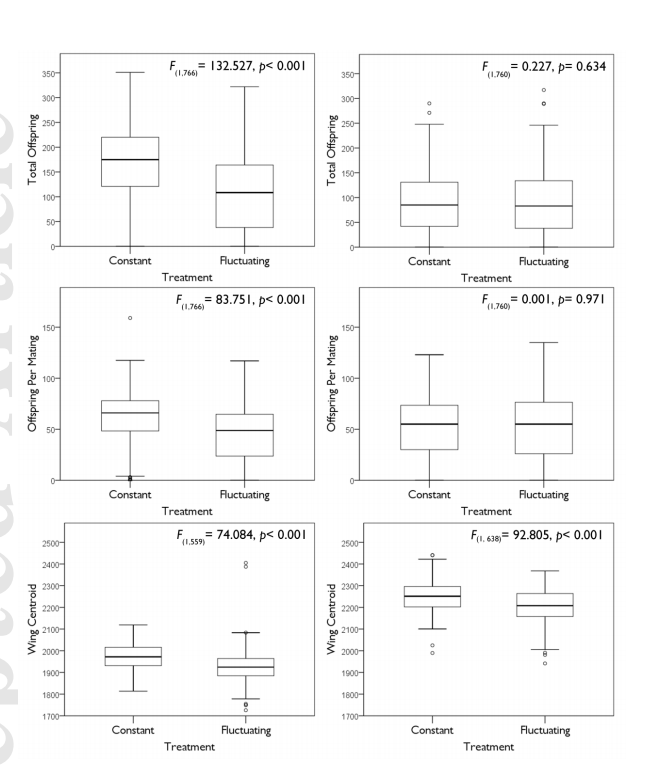
\includegraphics[width=1.05\linewidth]{figures/figure1} 

}

\caption[Metrics to describe and explain environmental variability.]{An example of environmental variability using diurnal light availability to model how range, mean, predictability, and duration can be used to characterize different patterns of variability. Shown is a comparison of how duration of variability compares within the same environmental factor. Terms highlighted in each panel are described below in the main text}\label{fig:unnamed-chunk-3}
\end{figure}
Environmental variability describes the dynamic characteristics of abiotic and biotic environmental conditions, in addition to how abiotic and biotic factors interact to drive organisms' response to environmental conditions (Gudmundson, Eklöf, \& Wennergren, 2015; Parepa, Fischer, \& Bossdorf, 2013). Though there are several characterized patterns of environmental variability (sinusoidal, stochastic, colored noise, reviewed below), patterns of variation can be further understood using the same core set of attributes: range, mean, duration, and predictability (Figure 1.1).

\hypertarget{mean}{%
\subsection{Mean}\label{mean}}

Aggregating values together, whether it be temperature, light availability, precipitation, allows for a better understanding of trends and patterns as opposed to random events. The mean can be used as a zeroing point for any environmental condition that we can use to compare across patterns, studies, and time. It provides a departure point for what we expect the average value to be for all time. In certain cases, the mean is a useful metric for observing trends by minimizing the noise of environmental conditions, i.e.~averaging population growth rates to understand if a disease is affecting organisms across geographic locations or just specific locations. However, in other cases, the mean is less useful compared to the variability. For instance, if there are key factors contributing to population growth rates from specific locations, comparing the amount of variability in additional variables across locations (individual respiration rates, temperature, etc.) is more fruitful for the task at this scale. At some point however, all data of interest are averages. The important distinction is the scale at which we average the data and the level of detail provided at each scale. Means are more useful in describing variation amongst normally distributed data, however, other statistical metrics like the median or mode may be more appropriate when the data is not normally distributed.

\hypertarget{amplituderange}{%
\subsection{Amplitude/Range}\label{amplituderange}}

We can expand additional information adjacent to the mean (i.e.~range, duration, predictability) for a finer scale picture of environmental conditions, as Vasseur et al outlined that increases in temperature variation posed a greater risk to species than just simply considering increases in global temperature (Vasseur et al., 2014). We can further quantify how variable an environment is by accounting for the range, or total span of conditions an organism may experience. This range can be short or long, for example, geographic location drastically influences the amount of sunlight an ecosystem receives. The Amazon Rainforest experiences less variation in light availability during the year than Denali National Park in Alaska, which experiences high variation in light availability between the summer and winter seasons. The range of environmental conditions an organism experiences can influence their ability to withstand changes in mean temperature (Amarasekare \& Coutinho, 2013; Amarasekare \& Savage, 2012), as well as additional life history traits (size, speed, etc.). An organism's ability to withstand changes in mean temperature has been attributed to the location of their optimal thermal temperature and the temperature at which survival is no longer possible (Amarasekare \& Savage, 2012). If an organism has an optimal temperature that is very close to that survival threshold, they are less able to adapt and withstand an upward thermal shift that occurs on a faster timescale than their adaptive evolution can manage.

\hypertarget{duration}{%
\subsection{Duration}\label{duration}}

The amount of time an organism spends at different conditions is also important for how we understand and describe environmental variability. Variability can be examined on many different scales, from daily changes in light availability to seasonal changes in light availability (Figure 1.1). Short term fluctuations, such as Fluctuating Thermal Regimes (FTR), in which an organism only experiences a change in temperature for a short period of time (less than one generation), have differing effects on performance (Colinet, Rinehart, Yocum, \& Greenlee, 2018). Performance is a set of whole organism traits (i.e.~assimilation, development, metabolic rate) with the availability to perform dynamics actions and tasks pertinent to fitness or organismal success and is often used as a way to estimate the culmination of organismal processes that hinder or help an organisms' persistence in the environment (Amarasekare \& Savage, 2012; Husak \& Lailvaux, 2017). While studies that employ FTR are doing so in an explicitly ecologically irrelevant context, as organisms reared in a cold environment do not usually experience warming exposures during a single day. However, there are instances in nature where organisms do experience short periods of extreme temperature changes (i.e.~heat waves, cold fronts, etc.) in which the benefits of FTR in mitigating chill injuries may be helpful. Beyond the period of fluctuation organisms experience, it is important to also consider how the period of fluctuation aligns with individual, population, and community level processes. For instance, Temperature-dependent Sex Determination (TSD), in which ectotherms rely on the environment to incubate their larval offspring, is greatly affected by temperature changes during a specific window of development (Bowden \& Paitz, 2018; Delmas, Prevot-Julliard, Pieau, \& Girondot, 2007). Further, at the population level, if organisms are closer or farther to carrying capacity, the impact of fluctuation may help or hinder population growth depending on the magnitude of variance (Lawson, Vindenes, Bailey, \& Pol, 2015). When considering community dynamics, similar effects may appear depending on when a fluctuation occurs in time relative to predator/prey dynamics (Bastille-Rousseau et al., 2018; Dobramysl \& Tauber, 2013; Romanuk \& Kolasa, 2002).

\hypertarget{predictability}{%
\subsection{Predictability}\label{predictability}}

FTR can also describe the predictability of the fluctuation period. Variability may not have evenly spaced intervals (i.e.~heat waves that occur at irregular intervals within a summer season), such that organisms can experience different amounts of variability for different amounts of time. Predictability can also attempt to describe stochastic vs.~autocorrelated variation, however, that will be discussed in a different context below (Figure 1.3).

\hypertarget{link-between-temporal-and-spatial-variability}{%
\subsection{Link between temporal and spatial variability}\label{link-between-temporal-and-spatial-variability}}

While not explicitly an area of study for this work, it is important to include how temporal and spatial variability can interact. Spatial variability describes how in three dimensional space, environments, organisms, and conditions can vary based on their location in space (Farhang-Sardroodi, Darooneh, Kohandel, \& Komarova, 2019; Horne \& Schneider, 1995). Spatial variability can interact with temporal variability in cases where organisms mitigate temporally variable conditions by modifying their spatial location, i.e.~Diel vertical migration (DVM). In DVM, organisms migrate to the surface and bottom of lakes based mainly on cues of light availability (Brierley, 2014; Lampert, 1989). However, there are also instances in which the environment is not temporally variable yet an organism utilizes spatial variability to regulate its behavior, i.e.~an organism moving from sun to shade during the day to regulate body temperature and metabolic processes (Huey, 1974; Kearney, Shine, \& Porter, 2009).

Though environmental variability can include many different forms, from fluctuations in resource availability
(Dempster \& Pollard, 1981; Sommer, 1984) to light (Morison, Franzè, Harvey, \& Menden‐Deuer, 2020; Ruel \& Ayres, 1999), one of the best studied and all-encompassing forms of fluctuations are thermal fluctuations (Colinet, Sinclair, Vernon, \& Renault, 2015; Huey \& Bennett, 1990).

\hypertarget{thermal-variability}{%
\section{Thermal variability}\label{thermal-variability}}

\hypertarget{what-is-temperature-variability}{%
\subsection{What is temperature variability?}\label{what-is-temperature-variability}}

Changes in temperature can be grouped into a couple different orientations, the first being the difference between the terms ``fluctuating'' and ``variation'' with respect to temperature. Though many studies have implicitly assumed the audience understands the distinction between the two terms, Colinet et al explicitly defined fluctuating temperature as ``a generic term that refers to any discontinuous thermal regime that occurs on a short-term basis'' (2018). Most generally, temperature variability describes changes in environmental temperature through time (Colinet et al., 2018; Holmes, Woollings, Hawkins, \& Vries, 2016).

\hypertarget{why-is-it-important-to-ecological-processes}{%
\subsection{Why is it important to ecological processes?}\label{why-is-it-important-to-ecological-processes}}

Most organisms experience and rely on temperature to regulate metabolic processes or signal a behavior or response to ultimately persist in the environment (Huey \& Bennett, 1990). Brown et al highlighted the importance of both temperature and body size in the metabolic theory of ecology (MTE) (Brown, Gillooly, Allen, Savage, \& West, 2004). Though highly debated (Clarke, 2006), MTE serves as an origin point for understanding how organisms respond to environmental conditions. MTE is described by the following equation:

\[
B = b_0M^{3/4}e^{-E/kT}
\]

Where \(B\) is organismal metabolic rate, \(b_0\) is a normalization constant unrelated to temperate or body size, \(M\) is organismal mass, and \(e^-E/kT\) is referred to as the ``Boltzman factor'', where \(E\) is activation energy, \(k\) is the Boltzman constant and \(T\) is temperature. Together, all of these values aim to describe the relationship between temperature and body size to determine metabolic rate. We assume that organismal level responses should scale across higher levels of organization, as MTE predicts that after correcting for body mass and temperature, metabolic rates should be the same. However, there are unexplained differences that the equation cannot fully explain, like heterogeneity in resting metabolic rate of teleost fish (Clarke, 2006; Clarke \& Johnston, 1999). Others believe that MTE makes valid assumptions and is more flexible than opponents argue, as it provides a foundational framework for general estimates of metabolic rate for larger, more generalizable taxonomic groups (Gillooly et al., 2006). Regardless of the debates about the details of MTE, at the very least, it provides a great foundation for thinking about temperature dependent processes.

MTE supports temperature impacting metabolic rate, which can have downstream effects on fitness characteristics. This is typically described by a characteristic unimodal, right skewed response that organisms typically demonstrate called a thermal performance curve (TPC) (Figure 1.2).
\begin{figure}

{\centering 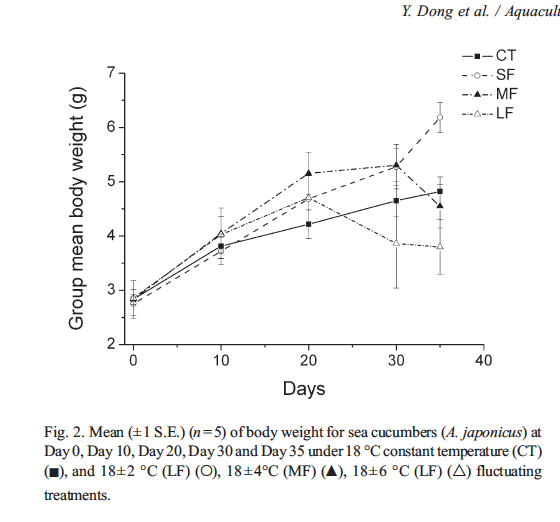
\includegraphics[width=0.9\linewidth]{figures/figure2} 

}

\caption[Thermal performance curve components]{Schematic of thermal performance curve and it’s important components for understanding thermal performance. Adapted from (Krenek et al 2012, Tuff et al 2016).}\label{fig:unnamed-chunk-4}
\end{figure}
The critical points that have been identified in thermal performance curves include: Thermal Optimum (Topt), Critical Thermal Minimum (CTmin), Critical Thermal Maximum (CTmax), Thermal tolerance breadth, and the Tolerance range. CTmin and CTmax describe the absolute limits of an organism's tolerance range, such that beyond these two thresholds, organisms' performance is negatively impacted (Brown et al., 2004; Dowd, King, \& Denny, 2015). Topt is the temperature at which performance is highest, and is importantly situated just before the sharp decline in performance that converges on CTmax.

TPCs non-linear shape represents the relationship between temperature and performance, such that performance is an amalgamation of many life history characteristics and biological processes (i.e.~metabolism) (Amarasekare \& Savage, 2012). If only temperature's effect on metabolism were considered, the shape of the relationship may be an exponential one. However, there are several other constraining factors (i.e.~energy acquisition, nutrient availability, etc.) that drive the characteristically nonlinear pattern of TPCs. TPCs strive to represent the complexity of many interacting processes an organism experiences in the environment with respect to thermal dependence, cementing their place as an important metric to conceptualize and understand temperature dependence.

\hypertarget{jensens-inequality-and-its-impacts-on-metabolic-rate}{%
\subsection{Jensen's Inequality and its impacts on metabolic rate}\label{jensens-inequality-and-its-impacts-on-metabolic-rate}}

TPCs have been crucial in predicting, understanding, and capitulating how organisms respond to their environment (Bernhardt, Sunday, Thompson, \& O'Connor, 2018). However, TPCs usually consist of measurements taken across an array of constant temperatures (i.e.~15-35°C in 5°C increments, with organisms reared at those temperatures constantly for the duration of an experiment to estimate thermal performance). These performance measurements are useful for a baseline understanding of thermal performance, however, they are not reflective of the variable conditions organisms experience in their environments.

Given the characteristically nonlinear shape of TPCs, Jensen's inequality is important in understanding the limits of thermal performance estimated under constant conditions versus variable conditions. Jensen's inequality describes the phenomenon that environmental variation can predictably and significantly impact nonlinear biological processes such that the consequences cannot be aptly inferred from average environmental conditions (Ruel \& Ayres, 1999). For instance, Ruel and Ayres provide the development rate of ectotherms as an example to demonstrate Jensen's inequality (Ruel \& Ayres, 1999). The development rate of ectotherms have a characteristically non-linear shape, such that responses increase at lower temperatures, become linear at intermediate temperatures, and decrease at higher temperatures (Ruel \& Ayres, 1999). With Jensen's inequality, we can predict that the effects of temperature variation will be positive at lower temperatures, neutral at intermediate temperatures, and negative at higher temperatures (Ruel \& Ayres, 1999). Given this, it is important to recognize that the constant temperatures used to generate TPCs are simply averages of environmental conditions during a moment in time. It is therefore reasonable to extrapolate that thermal performance under truly variable conditions may drastically differ and has been demonstrated by subsequent studies (Bernhardt et al., 2018; Khelifa et al., 2019).

Beyond accurately predicting how variable environmental conditions affect thermal performance, the bounds and critical points of TPCs are important for understanding how changes in environmental conditions may differentially impact different groups of organisms. For instance, Amarasekare et al 2012 demonstrated the importance where Topt is located relative to CTmax, such that ectotherms with a closer range between those two critical points at different geographic ranges may be negatively impacted by shifts in temperature and variability patterns (Amarasekare \& Savage, 2012; Paaijmans et al., 2013). Ectotherms in warm regions with an already minimized distance between Topt and CTmax may risk rapid extinction because there is less of a buffer to withstand increases in environmental temperature (Amarasekare \& Savage, 2012).

\hypertarget{relevancy-of-thermal-variability-in-the-modern-context}{%
\subsection{Relevancy of thermal variability in the modern context}\label{relevancy-of-thermal-variability-in-the-modern-context}}

Outside of the debate about the equations for determining metabolic rate, many of these equations rely on constant temperature conditions to predict metabolic rate. Variation in temperature is predicted to affect performance more significantly than increasing temperatures (Vasseur et al., 2014); thus, if there is disagreement about how metabolic rates scale across species, communities, and ecosystems, how might non-constant temperature alter predictions regarding performance? Khelifa et al demonstrated in five species from the same genus that when correcting for non-linearity, lab controlled experiments of diurnal variation in temperature and constant temperature did not differ significantly from one another in their thermal performance (Khelifa et al., 2019).

However, beyond diurnal or sinusoidal variation, there are other variation patterns at different timescales that all levels of biological organization experience (Figure 1.3). Khelifa et al demonstrated that when organisms are exposed to ambient temperatures in the environment, their thermal performance becomes less predictable (Khelifa et al., 2019). Beyond diurnal fluctuations in temperature, organisms can experience seasonal fluctuations as well as annual fluctuations in temperature. Vasseur and Yodzis outline how the frequency (1/period) of environmental fluctuations describes the ``color of environmental noise'' (Vasseur \& Yodzis, 2004). In colored noise, red noise describes lower frequencies and longer periods whereas white noise describes higher frequencies and shorter periods. Temperature is predicted to become more reddened or autocorrelated over time, meaning that temperatures will become more similar and predictable (Tabari, Hosseinzadeh Talaee, Ezani, \& Shifteh Some'e, 2012; Wigley, 1998). Understanding how organisms at all scales respond to these different patterns of variation in temperature is key for a more informed understanding of persistence.
\begin{figure}

{\centering 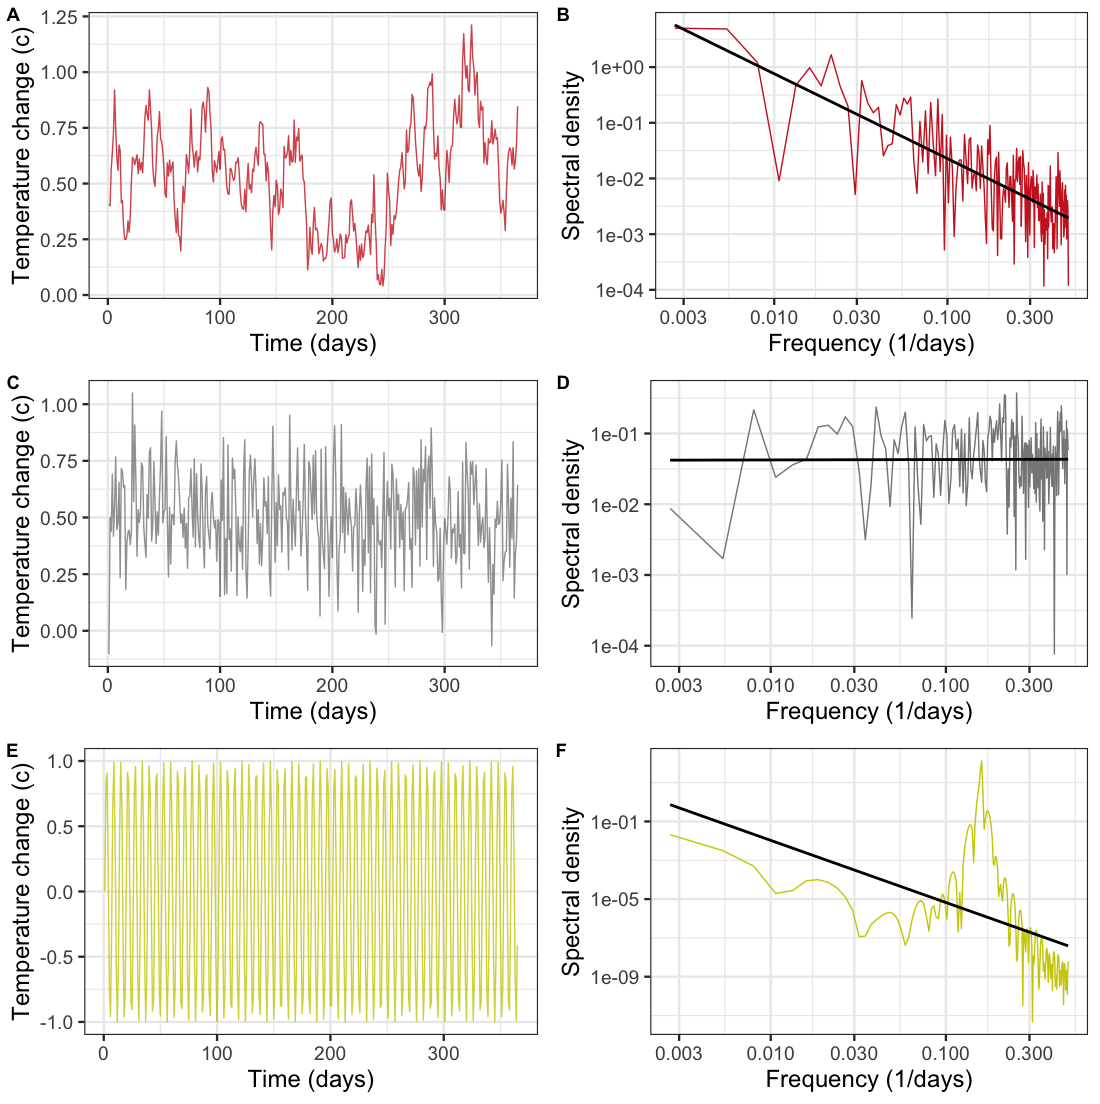
\includegraphics[width=0.9\linewidth]{figures/figure4} 

}

\caption[Patterns of variability and spectral density plots]{Time series of daily changes in autocorrelated (A), stochastic (C), and diurnal (E) temperature variation over one year, accompanied by the respective spectral density plots for each pattern of variation (B,D,F). Adapted from and inspired by Massey et al 2020 and Kroeker et al 2020.}\label{fig:unnamed-chunk-5}
\end{figure}
\clearpage

\hypertarget{objectives-driving-questions-hypotheses}{%
\section{Objectives, driving questions, hypotheses}\label{objectives-driving-questions-hypotheses}}

Thermal fluctuations are expected to have an effect on performance across the individual, population, and community level:
\begin{itemize}
\item
  At the individual level, this usually comes in the form of reduced fitness, increased development rates, and/or decreased physiological responses from reduced maximum temperatures, flattening the thermal performance curve (Bartheld, Artacho, \& Bacigalupe, 2017) to changes in TSD ratios (Bowden \& Paitz, 2018)
\item
  At the population level, this usually comes in the form of decreasing population densities (Anders \& Post, 2006)
\item
  At the community level, this usually comes in the form of promoting coexistence in the face of emigration (Descamps-Julien \& Gonzalez, 2005), or population success via inflationary effects (Holt et al., 2003)
\end{itemize}
It is, however, less understood how variation patterns influence these characteristic responses at each level of organization. Many individual level studies focus on responses to diurnal fluctuations in temperature, whereas higher levels of organization have explored how colored noise elicits these characteristic responses (Petchey, 2000).

There has yet to be a quantitative review of the effect of environmental variability across ecological scales, even though many studies have looked at variability (Kroeker et al., 2020; Massey, Holt, Brooks, \& Rollinson, 2019). To understand how environmental variability affects organisms, populations, and communities, we conducted a meta-analysis on the effects of thermal variability on responses across different levels of biological organization to answer the following questions: 1) Does variability pattern drive differences in response magnitude? (i.e.~does autocorrelated variation have a larger impact on response than stochastic or diurnal variation?), 2) Does temperature variability drive differential response levels at different levels of biological organization?, 3) How can the magnitude of response be influenced by additional factors (i.e.~periodicity, age, size, thermal history, etc.)? We aim to answer these questions by collecting data from the literature at different levels of biological organization to systematically analyze responses across levels of organization.

We hypothesize that: 1) The larger the range of temperatures an organism will experience relative to their thermal performance curve will negatively impact the magnitude of response (full model), 2) Additional covariates related to biological fitness and success, experimental age and organism size will be correlated with negative responses, such that older organisms will cope better and smaller organisms will cope worse with increased thermal variability (full model), 3) Across organization levels, individual level studies will experience decreased performance compared to population level studies and higher levels of organization due to their ability to mitigate and rescue performance with population dynamics (full model), 4) If organisms experience temperatures that exceed their Topt, their responses will be negatively impacted (thermal stress model).

\hypertarget{methods}{%
\chapter{Methods}\label{methods}}
\begin{figure}

{\centering 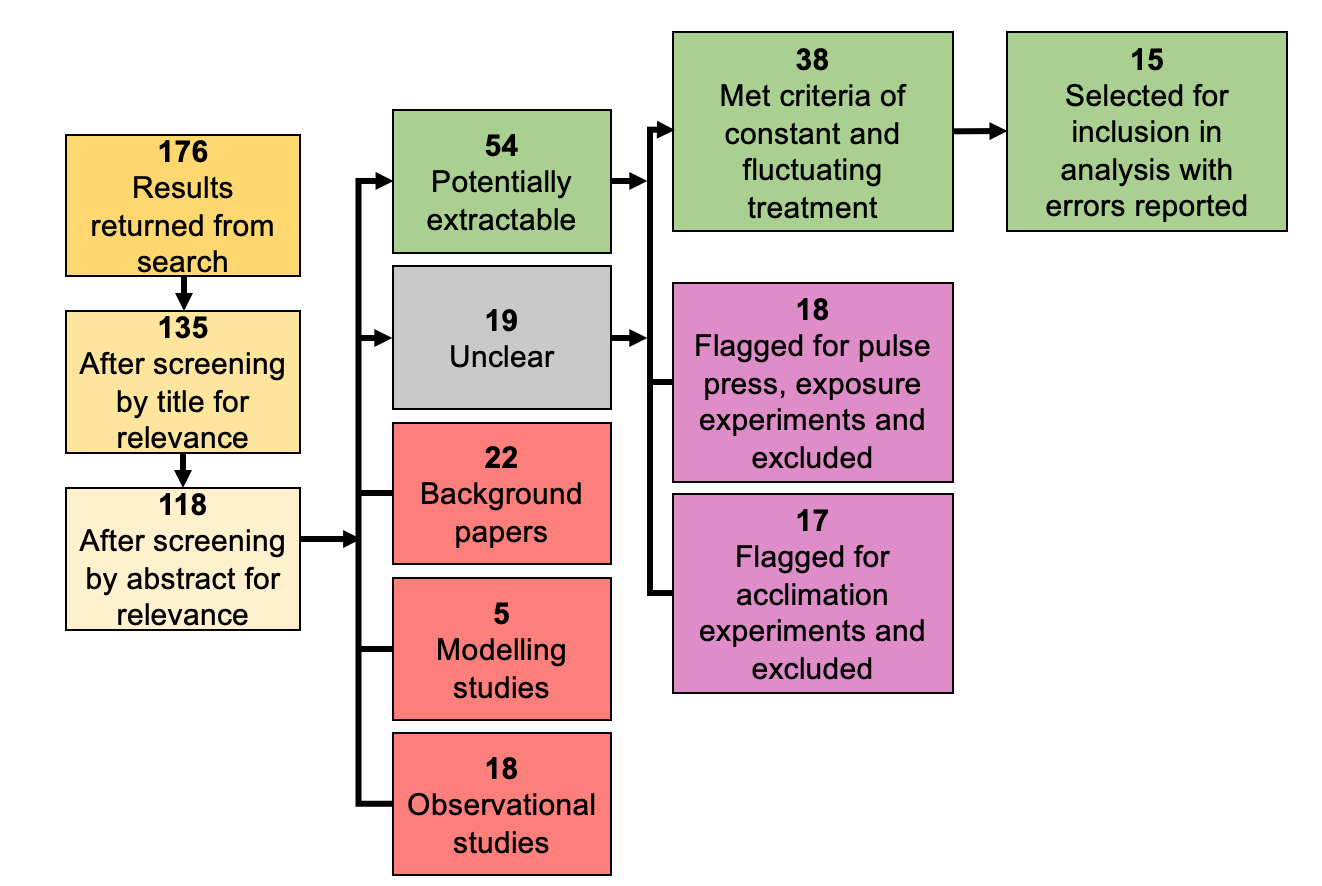
\includegraphics[width=0.9\linewidth]{figures/figure5} 

}

\caption[Meta-analysis paper selection process]{Diagram of the paper selection process from the original 176 papers returned from the Web of Science search to the 19 studies included in the analysis. Red indicates no usable data, purple indicates some usable data but not for our study questions, and green indicates usable data flow for inclusion in analysis.}\label{fig:unnamed-chunk-7}
\end{figure}
We conducted a systematic literature search using the ISI Web of Science database to collect studies that investigated the effects of temperature variability (Figure 2.1). After trying several different combinations of search terms to capture research on temperature variability, our final search utilized these search terms in an advanced search: AK=((temperature OR thermal) NEAR (vari* OR fluc*)) AND SU=(Life Sciences \& Biomedicine). This search returned a total of 176 results. We downloaded the .bib file of this search and imported this file into the revtools R package (version 0.4.1). Using the revtools package we then screened studies by title, then by abstract, for inclusion in analysis (Figure 2.1). Once we screened studies for relevance to the field of biology and environmental variation, we began excluding studies using the following strict criteria:
\begin{itemize}
\tightlist
\item
  We excluded studies that did not feature both a constant and fluctuating treatment (i.e.~studies with several fluctuating treatments but no constant comparison or studies with a gradient of constant treatment temperatures but no periodic fluctuating treatment)
\item
  We excluded studies that were not completed in a laboratory (i.e.~modeling predictions or results from models, mesocosm experiments, in situ experiments)
\item
  We excluded studies in which the responses were measured in different thermal conditions than the incubation or rearing thermal conditions (i.e.~organisms reared in fluctuating temperatures, but measured responses at different constant temperatures to yield a thermal performance curve (TPC))
\item
  We excluded any articles not written in English
\item
  We excluded studies that did not report measurements of error
\item
  We excluded studies in which the response variables are comparable or extractable (i.e.~one study performed Principal component analysis for their responses)
\end{itemize}
We excluded studies that did not have the same mean for constant and fluctuating treatments (i.e.~treatments at the minimum and maximum with a fluctuation treatment across the range) or a mean within 1°C of the two treatments. We chose to exclude studies that did not match this criteria as there would not have been a baseline comparison to attribute changes in response magnitude to most simply variation, as changes in mean temperature significantly influence the magnitude of response (Brown et al., 2004). The final number of data points included in the analysis is broken down by study (Table 2.1).

\clearpage
\begin{table}[!h]

\caption[Studies included in analysis of thermal variability]{\label{tab:unnamed-chunk-8}Studies included in analysis of thermal variability (n=15)}
\centering
\begin{tabular}[t]{lll}
\toprule
\textbf{Study} & \textbf{Year} & \textbf{Extracted data points (n)}\\
\midrule
\cellcolor{gray!6}{Delava et al} & \cellcolor{gray!6}{2016} & \cellcolor{gray!6}{16}\\
Du et al & 2009 & 32\\
\cellcolor{gray!6}{Garcia-Ruiz et al} & \cellcolor{gray!6}{2011} & \cellcolor{gray!6}{16}\\
Glass et al & 2009 & 16\\
\cellcolor{gray!6}{Kern et al} & \cellcolor{gray!6}{2015} & \cellcolor{gray!6}{24}\\
\addlinespace
Kern et al & 2014 & 4\\
\cellcolor{gray!6}{Lowenborg et al} & \cellcolor{gray!6}{2012} & \cellcolor{gray!6}{10}\\
Maneti et al & 2014 & 24\\
\cellcolor{gray!6}{Pendlebury et al} & \cellcolor{gray!6}{2004} & \cellcolor{gray!6}{16}\\
Qu et al & 2014 & 40\\
\addlinespace
\cellcolor{gray!6}{Rolandi et al} & \cellcolor{gray!6}{2018} & \cellcolor{gray!6}{4}\\
Saxon et al & 2017 & 12\\
\cellcolor{gray!6}{Semenov et al} & \cellcolor{gray!6}{2007} & \cellcolor{gray!6}{32}\\
Simoncini et al & 2019 & 30\\
\cellcolor{gray!6}{Treidel et al} & \cellcolor{gray!6}{2015} & \cellcolor{gray!6}{4}\\
\bottomrule
\end{tabular}
\end{table}
\hypertarget{data-extraction-and-analysis}{%
\section{Data extraction and analysis}\label{data-extraction-and-analysis}}

From the studies that met our inclusion criteria, we extracted data from tables and figures. Figures were extracted via .png files imported into WebPlotDigitizer to obtain the raw data. The extracted data was then imported into a master spreadsheet of data from all studies for analysis. We extracted mean values for response variables, any measure of variance (Standard Deviation (SD) or Standard Error of the Mean (SEM)), and sample size. For studies that reported error as SEM, we converted SEM to SD by multiplying the SEM by the square root of the same SEM. We also collected information on mean temperature, fluctuation range, organization level, body size, life stage, response type, thermal stress, and aggregated these values (Table 2.2).

If studies reported findings using medians and the Interquartile Range (IQR) via boxplots, a normal distribution of the data was assumed and a subsequent calculation was performed, such that the median is the mean and the IQR is the SD with a conversion calculation (Higgins et al., 2011). Lastly, if extracted values were missing variance or sample size estimates, the points were automatically excluded via the data analysis software, metafor.

\clearpage
\begin{table}[!h]

\caption{\label{tab:unnamed-chunk-9}Covariates included in models}
\centering
\begin{tabular}[t]{l>{\raggedright\arraybackslash}p{8cm}}
\toprule
\textbf{Variable} & \textbf{Description}\\
\midrule
\cellcolor{gray!6}{mean\_temp\_constant} & \cellcolor{gray!6}{Reported mean temperature (°C) in study}\\
flux\_range & Reported range (difference between minimum 
                                     and maximum) of temperature fluctuation (°C) experienced\\
org\_level & Level of biological organization, categorized
                                     as either 0 for individual or 1 for population level
\cellcolor{gray!6}{                                     responses}\\
size & Size estimate of study organism, 0 for extra-small (less than 1mm),
                                     1 for small (less than 5 cm), 2 for medium (less than 0.3 m), and 3
                                     for large (greater than 0.3 m)\\
exp\_age & Life stage at which experiment was conducted, 
                                     categorized as 0 for larval, 1 for juvenile (not sexually mature),
\cellcolor{gray!6}{                                     and 2 for adult}\\
\addlinespace
resp\_type & Response variable units classified as rates or traits, 
                                     such that rates included any response variable units with a
                                     “per day” clarifier, all else as traits\\
stressful & Whether or not the organisms experienced thermally stressful 
                                     temperatures throughout study duration, if temperature range 
                                     exceeded Topt, classified as thermally stressful, else not
                                     thermally stressful. See Appendix Table 1 for references in which
\cellcolor{gray!6}{                                     organisms’ thermal stress metrics were included}\\
\bottomrule
\end{tabular}
\end{table}
\clearpage

\hypertarget{metafor}{%
\section{Metafor}\label{metafor}}

We utilized metafor (version 2.4.0) in R to analyze the extracted, aggregated data. Metafor builds on the functionality of older meta-analysis packages (meta, etc.) by allowing for greater flexibility in model types (mixed and random effects models) (Viechtbauer, 2010). In order to use metafor, the package requires the data to be in a wider format, in which data are input into the following columns:
\begin{table}[!h]

\caption{\label{tab:unnamed-chunk-10}Column names expanded to wider format for data analysis in metafor}
\centering
\begin{tabular}[t]{ll}
\toprule
\textbf{Column name} & \textbf{Purpose}\\
\midrule
\cellcolor{gray!6}{Mf} & \cellcolor{gray!6}{Mean of experimental group}\\
SDf & Standard deviation of the experimental group\\
\cellcolor{gray!6}{Mc} & \cellcolor{gray!6}{Mean of the control group}\\
SDc & Standard deviation of the control group\\
\cellcolor{gray!6}{Nf} & \cellcolor{gray!6}{Sample size (n) of the experimental group}\\
\addlinespace
Nc & Sample size (n) of the control group\\
\bottomrule
\end{tabular}
\end{table}
\linebreak

Formatting the data in this way allows for metafor to calculate an effect size and sampling variance for each row in the dataset, such that a constant treatment and corresponding fluctuating treatment will be paired together using the \texttt{escalc} function in metafor to calculate effect size and sampling variance:
\begin{Shaded}
\begin{Highlighting}[]
\KeywordTok{escalc}\NormalTok{(}\DataTypeTok{measure=}\StringTok{"SMD"}\NormalTok{, }\DataTypeTok{m1i=}\StringTok{`}\DataTypeTok{constant_resp}\StringTok{`}\NormalTok{, }\DataTypeTok{m2i=}\NormalTok{flux_resp, }
            \DataTypeTok{sd1i=}\StringTok{`}\DataTypeTok{SD_constant}\StringTok{`}\NormalTok{, }\DataTypeTok{sd2i=} \StringTok{`}\DataTypeTok{SD_variable}\StringTok{`}\NormalTok{, }\DataTypeTok{n1i=}\NormalTok{constant_samp, }
       \DataTypeTok{n2i=}\NormalTok{flux_samp, }\DataTypeTok{data=}\NormalTok{dat_MA, }\DataTypeTok{slab=}\KeywordTok{paste}\NormalTok{(study_id, experiment_id, }
\NormalTok{                                              response_id, }\DataTypeTok{sep=}\StringTok{", "}\NormalTok{))}
\end{Highlighting}
\end{Shaded}
We specified the effect size metric of interest to be the standardized mean difference (SMD), as this is a common calculation used to compare two groups head to head (Viechtbauer, 2010). It is also a powerful metric to use in a meta-analysis because it standardizes the responses across studies to reduce heterogeneity and bias (Viechtbauer, 2010). Each of the subsequent arguments of the \texttt{escalc} function specify the mean, standard deviation, and sample size for each paired constant and fluctuating treatment. The \texttt{escalc} function is using multiple equations to ultimately output the SMD and sampling variance, all of which are below (Figure 2.2).
\begin{figure}
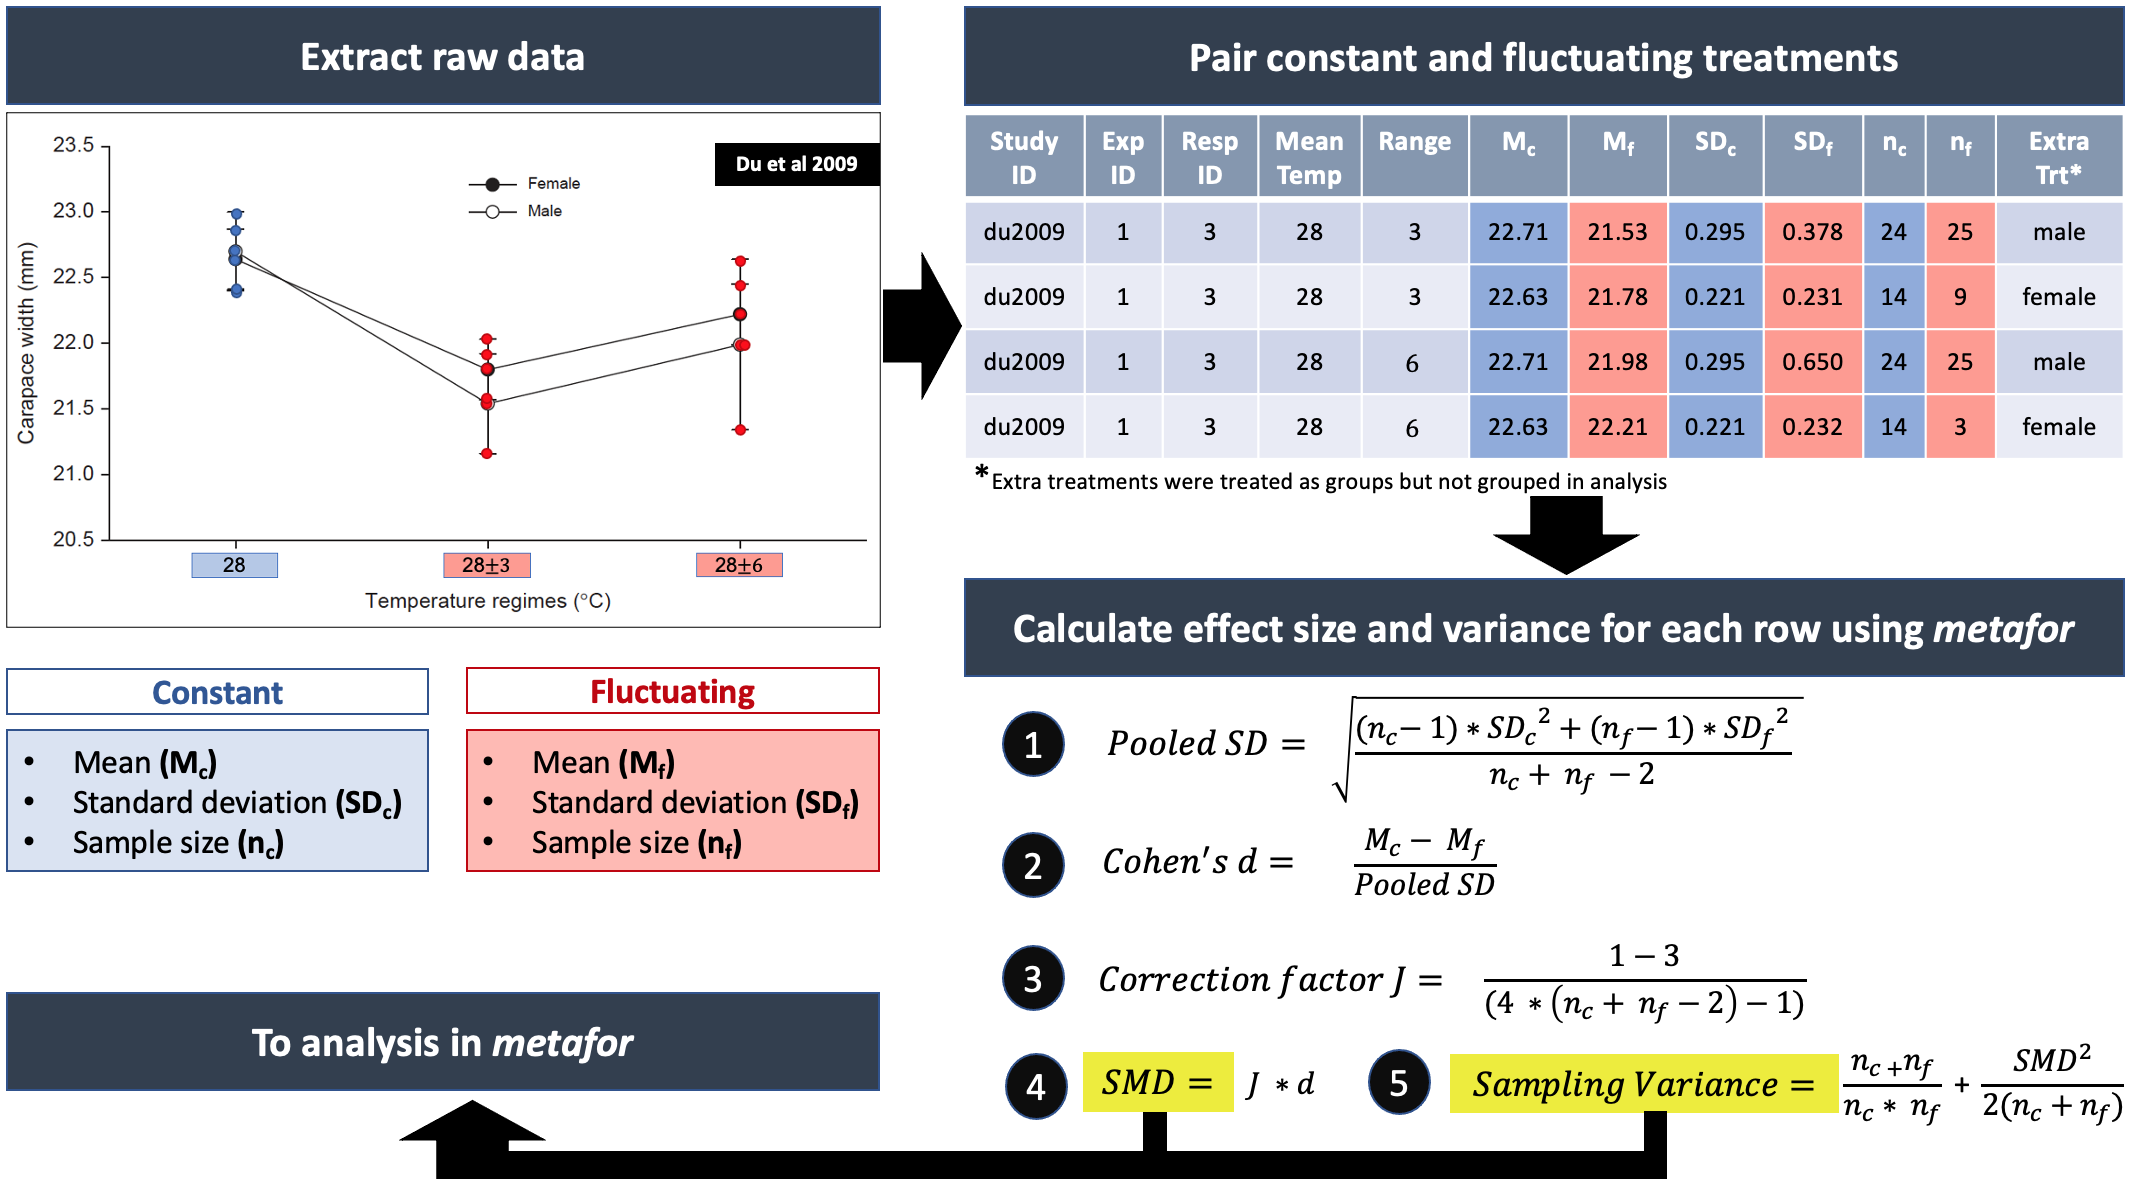
\includegraphics[width=1\linewidth]{figures/figure6} \caption[Workflow of analysis in metafor]{Workflow diagram of how data were extracted, analyzed, and processed for downstream analysis in metafor.}\label{fig:unnamed-chunk-12}
\end{figure}
First, it calculates the pooled standard deviation (Pooled SD) from the sample sizes of both studies. Our data had studies with a wide range of sample sizes, so we wanted to include separate sample sizes between the constant and fluctuating treatments. The Pooled SD, Cohen's d, which is one of the most common ways to measure effect size, is used to normalize the mean differences between constant and fluctuating treatments. Then, using a correction factor J, which again normalizes the data further, we obtain the final SMD. The SMD is then ultimately used to calculate the sampling variance, which creates a unitless metric for variance.

Both the SMD and sampling variance are then input into the \texttt{rma.mv} function in metafor to generate a multivariate random effects model to understand how variability compares across studies and what factors may influence the magnitude of response. We first ran a multivariate random effects model without modifiers (simple model) to establish baseline heterogeneity between studies to then examine modifiers that could better explain the heterogeneity in effect sizes across studies:
\begin{Shaded}
\begin{Highlighting}[]
\KeywordTok{rma.mv}\NormalTok{(yi, vi, }
       \DataTypeTok{data=}\NormalTok{dat_MA_ES, }
       \DataTypeTok{random =} \OperatorTok{~}\DecValTok{1} \OperatorTok{|}\StringTok{ }\NormalTok{study_id }\OperatorTok{/}\StringTok{ }\NormalTok{experiment_id}\OperatorTok{/}\StringTok{ }\NormalTok{response_id, }
       \DataTypeTok{method=}\StringTok{"REML"}\NormalTok{) }
\end{Highlighting}
\end{Shaded}
The arguments of the \texttt{rma.mv} function include SMD (yi), sampling variance (vi), the datafile, as well the random argument to specify the structure of the model. We specified a nested structure to account for the colinearity of data points from within the same study, experiment, and response metric. We used Restricted Maximum-Likelihood (REML) to specify the fit of the model, as REML is best at handling small samples sizes compared to Maximum Likelihood (ML) (Viechtbauer, 2010). We chose a random effects model as opposed to a fixed effects model because we were interested in better understanding the patterns of the larger population of environmental variability literature, as we assumed the studies that were included in this analysis to be a random selection from the true population (Viechtbauer, 2010). The random effects model structure also allowed us to account for the nested structure of responses, experiment, and study to address the dependence of observations from within each study. The multivariate random effects model with all modifiers (full model) we ran included:
\begin{Shaded}
\begin{Highlighting}[]
\KeywordTok{rma.mv}\NormalTok{(yi, vi, }\DataTypeTok{data=}\NormalTok{dat_MA_ES, }\DataTypeTok{mods =} \OperatorTok{~}\NormalTok{flux_range }\OperatorTok{*}\StringTok{ }\NormalTok{mean_temp_constant }
       \OperatorTok{+}\StringTok{ }\NormalTok{exp_age }\OperatorTok{+}\StringTok{ }\NormalTok{size }\OperatorTok{+}\StringTok{ }\NormalTok{org_level }\OperatorTok{+}\StringTok{ }\NormalTok{resp_type, }
               \DataTypeTok{random =} \OperatorTok{~}\DecValTok{1} \OperatorTok{|}\StringTok{  }\NormalTok{study_id}\OperatorTok{/}\StringTok{ }\NormalTok{experiment_id}\OperatorTok{/}\StringTok{ }\NormalTok{response_id,}
                 \DataTypeTok{method=}\StringTok{"REML"}\NormalTok{) }
\end{Highlighting}
\end{Shaded}
The full model also included an interaction term between mean temperature and fluctuation range to understand if mean temperature coupled with fluctuation range was an important component in explaining patterns of variation. If an organism experiences large fluctuations in temperature range at a high mean temperature, it is more likely to exceed an organisms' Topt and become thermally stressful.

We decided to exclude the thermally stressful covariate as an argument in the full model because we lacked thermal stress data for one study. That particular study happened to be very influential in our model but the data was not misrepresented, as the data was extracted from a table (Garcia-Ruiz et al 2011, Table 1). The multivariate random effects model with all the covariates in the full model as well as thermal stress (exclusion model), which excluded Garcia-Ruiz et al 2011 entirely, included:
\begin{Shaded}
\begin{Highlighting}[]
\KeywordTok{rma.mv}\NormalTok{(yi, vi, }\DataTypeTok{data=}\NormalTok{dat_MA_ES, }\DataTypeTok{mods =} \OperatorTok{~}\NormalTok{flux_range }\OperatorTok{*}\StringTok{ }\NormalTok{mean_temp_constant }
       \OperatorTok{+}\StringTok{ }\NormalTok{exp_age }\OperatorTok{+}\StringTok{ }\NormalTok{size }\OperatorTok{+}\StringTok{ }\NormalTok{org_level }\OperatorTok{+}\StringTok{ }\NormalTok{resp_type }\OperatorTok{+}\StringTok{ }\NormalTok{stressful, }
               \DataTypeTok{random =} \OperatorTok{~}\DecValTok{1} \OperatorTok{|}\StringTok{  }\NormalTok{study_id}\OperatorTok{/}\StringTok{ }\NormalTok{experiment_id}\OperatorTok{/}\StringTok{ }\NormalTok{response_id,}
                 \DataTypeTok{method=}\StringTok{"REML"}\NormalTok{) }
\end{Highlighting}
\end{Shaded}
We also ran a separate model without this study and included the thermal stress covariate separately from all the other modifiers (thermal stress model) to see if thermal stress was truly an important factor or if it was simply excluding those influential data points:
\begin{Shaded}
\begin{Highlighting}[]
\KeywordTok{rma.mv}\NormalTok{(yi, vi, }\DataTypeTok{data=}\NormalTok{dat_MA_ES, }\DataTypeTok{mods =}  \OperatorTok{~}\StringTok{ }\NormalTok{stressful, }
               \DataTypeTok{random =} \OperatorTok{~}\DecValTok{1} \OperatorTok{|}\StringTok{ }\NormalTok{experiment_id}\OperatorTok{/}\StringTok{ }\NormalTok{study_id}\OperatorTok{/}\StringTok{ }\NormalTok{response_id,}
                 \DataTypeTok{method=}\StringTok{"REML"}\NormalTok{) }
\end{Highlighting}
\end{Shaded}
\hypertarget{results}{%
\chapter{Results}\label{results}}
\begin{figure}

{\centering 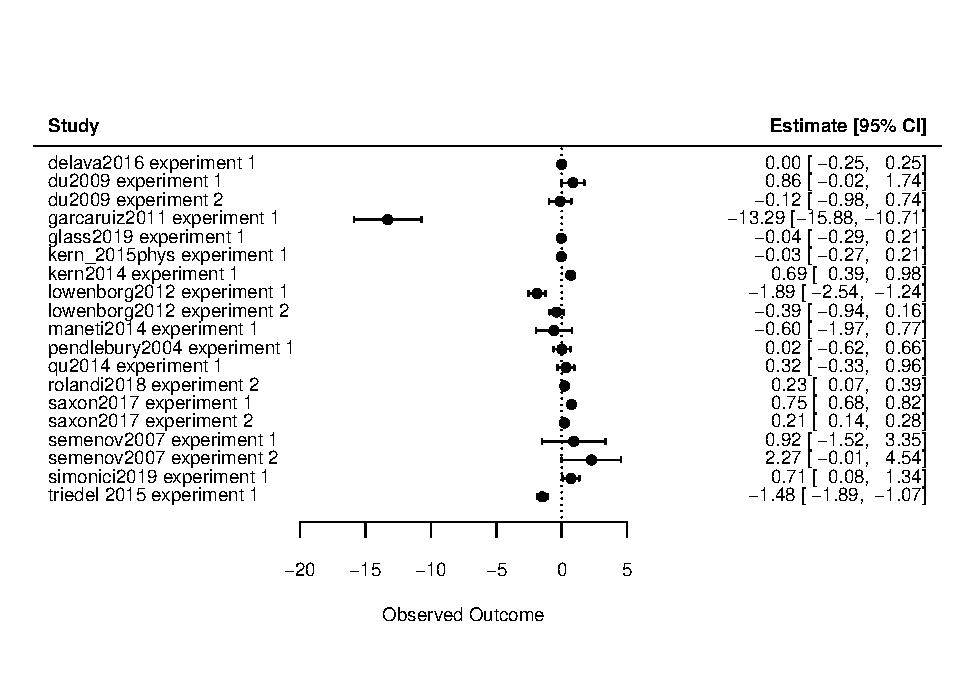
\includegraphics[width=0.95\linewidth]{thesis_files/figure-latex/unnamed-chunk-18-1} 

}

\caption[Forest plot of effect sizes]{Forest plot of effects sizes by study and experiment within a study. Indicates that both within and across studies, there were a wide range of effect sizes, likely due to experimental design (including fluctuation range, mean temperature, etc.) Each point represents an average of SMD for multiple responses within each experiment in a single study. Accordingly, the error bars represent an average of variance across multiple responses within a single experiment.}\label{fig:unnamed-chunk-18}
\end{figure}
Overall, even our simple model (n=140) demonstrates that the intercept is not significant but there was significant heterogeneity across studies (z= 0.79, p \textless{} 0.0001), as demonstrated by Figure 3.1. These results allow us to reject the null hypothesis that there are no significant differences between SMD across the studies included in analysis (see Appendix Figure 1). As was referenced in the methods, this allowed us to proceed in further detail how different covariates were influencing the effect sizes specifically.

Our full model, including 7 covariates (all, an additional interaction term between fluctuation range and mean temperature, and excluding thermal stress), responses were still significantly different from each other when accounting for the nested structure of responses, experiments, and studies (QM = 191.3722, df = 7, p \textless{} 0.0001). Further, fluctuation range (n=140) and the interaction term between fluctuation range and mean temperature (n=140) were statistically significant in the model (df = 7, p \textless{} 0.00001). Organization level (n=140) was also important in the model, as a statistically significant covariate (df= 7, p \textless{} 0.05).
\begin{figure}

{\centering 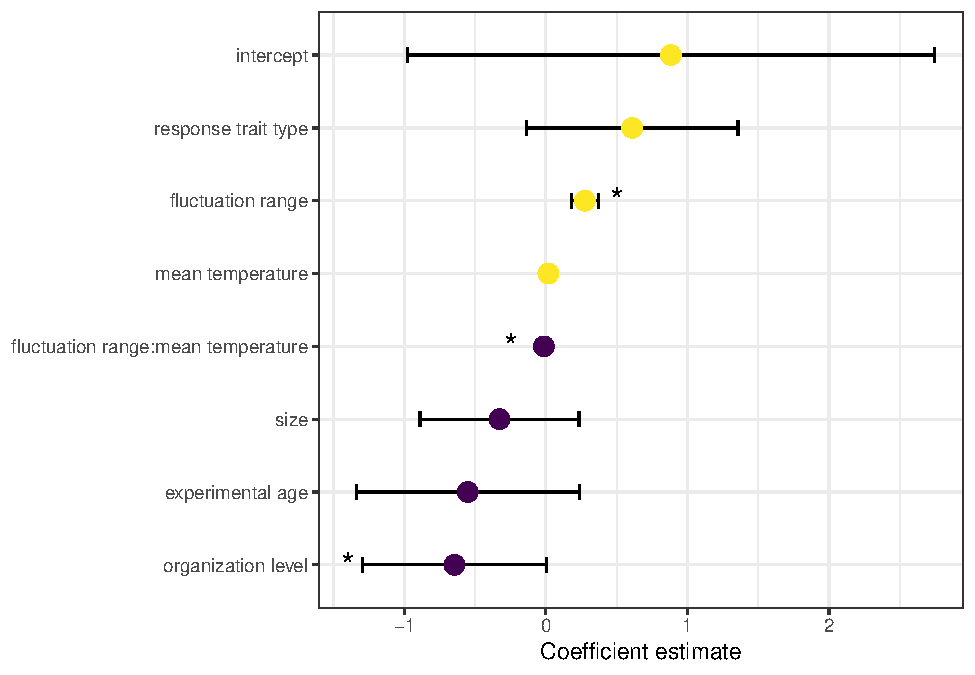
\includegraphics[width=0.95\linewidth]{thesis_files/figure-latex/unnamed-chunk-19-1} 

}

\caption[Coefficient estimates for full model]{Coefficient estimates for each covariate in the full model, where asterix symbols signify statistically significant model predictors.  Error bars represent 95 percent confidence intervals.}\label{fig:unnamed-chunk-19}
\end{figure}
\clearpage

Fluctuation range (n=140) had a positive estimate while the interaction term between range and mean temperature was only slightly negative, both of which were statistically significant at the p \textless{} 0.001 level (Figure 3.2). The most negative estimate, organization level (n=140), was significantly influential in our model at a significance level of p \textless{} 0.05. Surprisingly, the additional negative estimates of our model coefficients, experimental age (n=140) and size (n=140), were not statistically significant. In our analysis of thermal stress via a separate random effects model, we found thermal stress (n=132) was not statistically significant (df=1, p =0.4855) in explaining the effect size (Table 3.1).
\begin{table}[!h]

\caption[Thermal stress model summary statistics]{\label{tab:unnamed-chunk-20}Model summary statistics for random effects model using thermal stress as sole modifier}
\centering
\begin{tabular}[t]{lrrrrrr}
\toprule
\textbf{Term} & \textbf{estimate} & \textbf{se} & \textbf{zval} & \textbf{pval} & \textbf{ci.lb} & \textbf{ci.ub}\\
\midrule
\cellcolor{gray!6}{intercept} & \cellcolor{gray!6}{0.2050} & \cellcolor{gray!6}{0.1846} & \cellcolor{gray!6}{1.1104} & \cellcolor{gray!6}{0.2668} & \cellcolor{gray!6}{-0.1568} & \cellcolor{gray!6}{0.5669}\\
stressful & -0.0489 & 0.0702 & -0.6975 & 0.4855 & -0.1864 & 0.0886\\
\bottomrule
\end{tabular}
\end{table}
\clearpage

The interaction between fluctuation range and mean temperature as well as fluctuation range is best displayed in Figure 3.3. At lower mean temperatures, higher fluctuation ranges have a more positive effect on organism responses and performance, though that trend starkly ends at about \(24^{\circ}\)C. Beyond \(24^{\circ}\)C, the effect size decreases to nearly half the size of colder temperatures and hovers just above an effect size of one (Figure 3.3).
\begin{figure}

{\centering 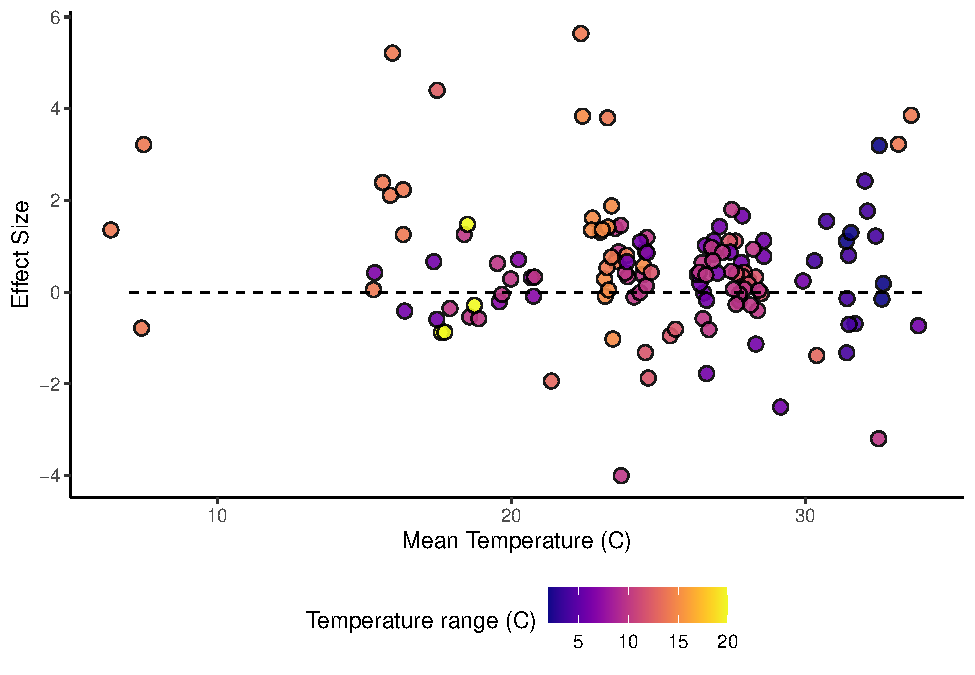
\includegraphics[width=0.9\linewidth]{thesis_files/figure-latex/unnamed-chunk-21-1} 

}

\caption[Scatterplot of relationship between range, mean, and effect size]{Scatterplot describing the relationship between mean temperature, temperature fluctuation range, and effect size. Temperature fluctuation ranged from 0-20°C, Mean temperature ranged from 7-33°C. Effect size ranged from -4 to 6, restricted based on the distribution of effect sizes to minimize impact of outliers (see Appendix Figure 2).}\label{fig:unnamed-chunk-21}
\end{figure}
The trend between organization level and temperature fluctuation range, suggests that populations perform better at higher fluctuation ranges than organisms (Figure 3.4). Interestingly, there were not any significant differences between thermal stress (Figure 3.5), life history metric (Figure 3.6), body size (Figure 3.7), or age (Figure 3.8).

As noted in the methods, when we excluded one highly influential study and included thermal stress in the exclusion model (n=132), size became much more important in the exclusion model (df=8, p \textless{} 0.001) as did mean temperature (df=8, p \textless{} 0.001). Surprisingly, organization level, fluctuation range, and the interaction between fluctuation range and mean temperature became insignificant in the exclusion model (df=8, p \textless{} 0.1).
\begin{figure}

{\centering 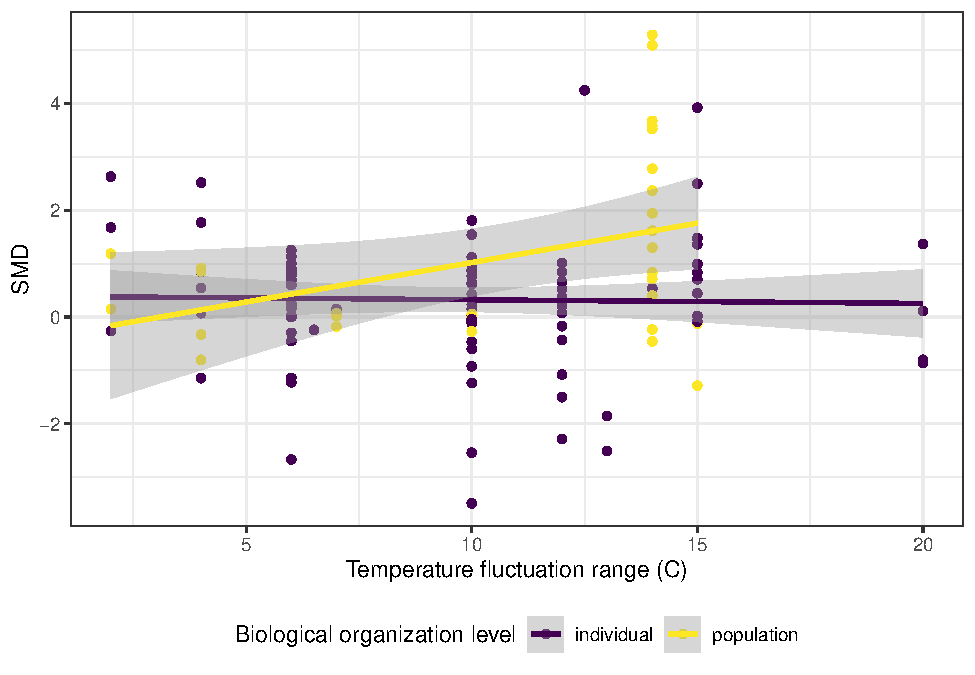
\includegraphics[width=0.85\linewidth]{thesis_files/figure-latex/unnamed-chunk-22-1} 

}

\caption[Effect sizes across temperature range by organization level]{Linear regression of SMD across temperature fluctuation ranges from 0 to 20°C, colored by organization level: individual or population level responses reported in studies.}\label{fig:unnamed-chunk-22}
\end{figure}
\clearpage
\begin{figure}

{\centering 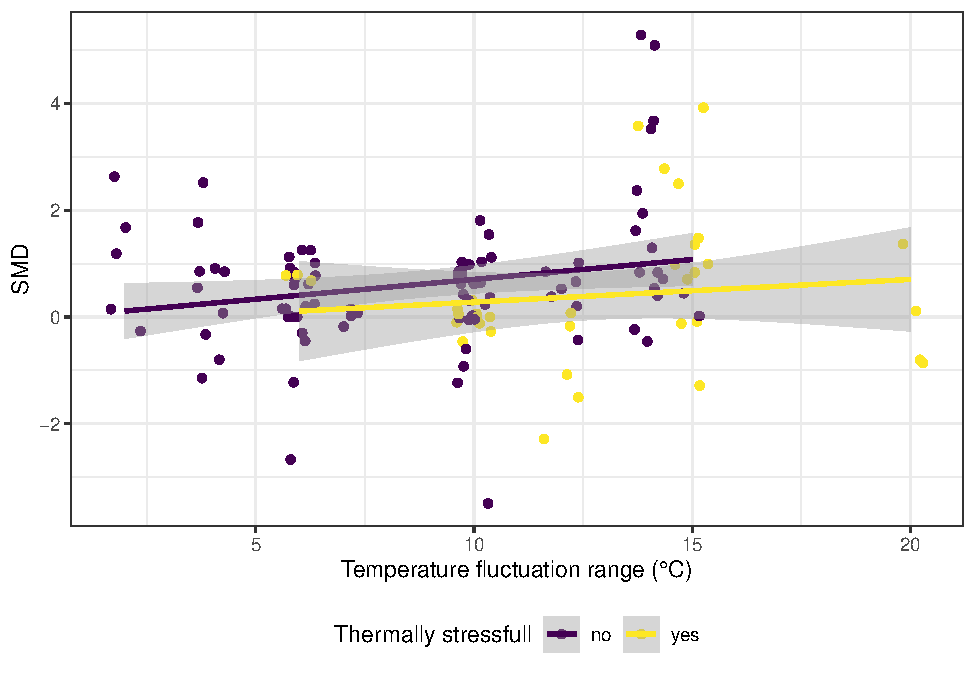
\includegraphics[width=0.85\linewidth]{thesis_files/figure-latex/unnamed-chunk-23-1} 

}

\caption[Effect sizes across temperature range by thermal stress]{Linear regression of SMD across temperature fluctuation ranges from 0 to 20°C, colored by thermal stress.}\label{fig:unnamed-chunk-23}
\end{figure}
\begin{figure}

{\centering 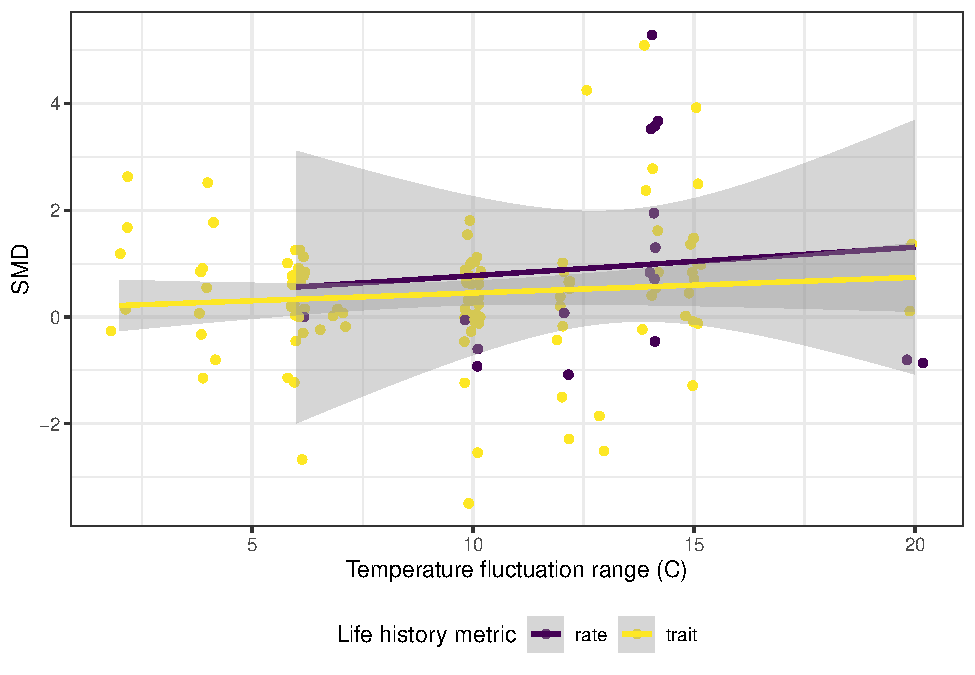
\includegraphics[width=0.85\linewidth]{thesis_files/figure-latex/unnamed-chunk-24-1} 

}

\caption[Effect sizes across temperature range by response type]{Linear regression of SMD across temperature fluctuation ranges from 0 to 20°C, colored by life history metric: responses categorized as rate or trait.}\label{fig:unnamed-chunk-24}
\end{figure}
\begin{figure}

{\centering 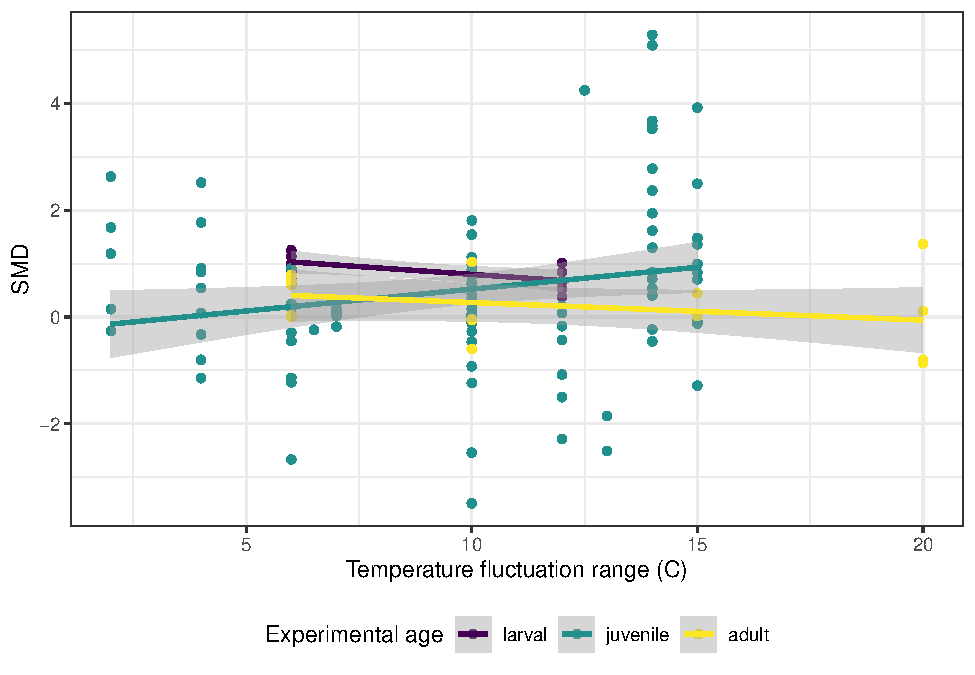
\includegraphics[width=0.85\linewidth]{thesis_files/figure-latex/unnamed-chunk-25-1} 

}

\caption[Effect sizes across temperature range by body size]{Linear regression of SMD across temperature fluctuation ranges from 0 to 20°C, colored by body size: extra-small, small, medium, or large.}\label{fig:unnamed-chunk-25}
\end{figure}
\begin{figure}

{\centering 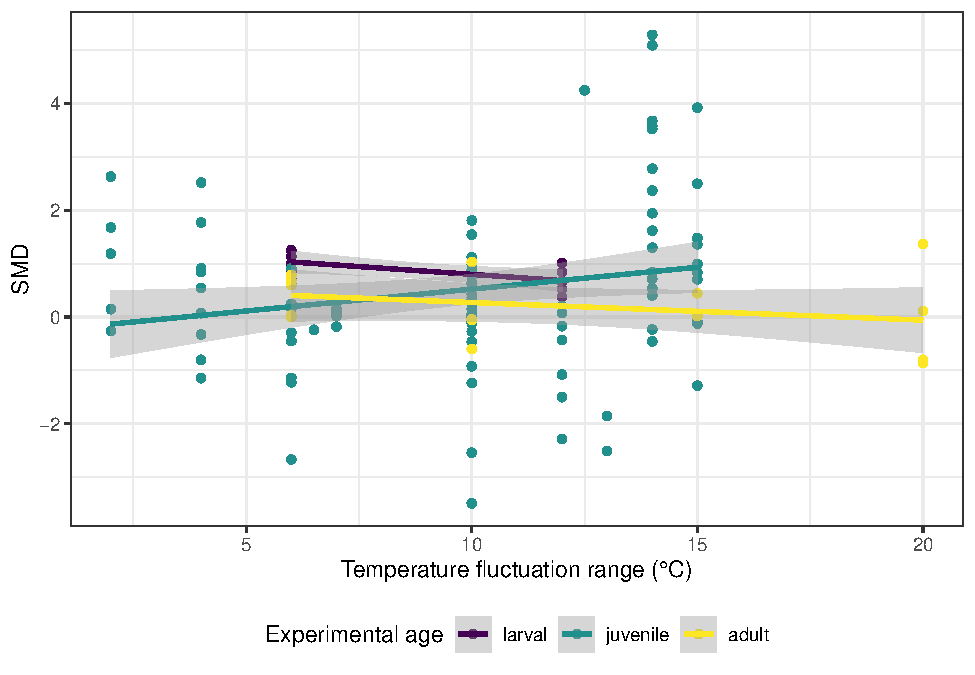
\includegraphics[width=0.85\linewidth]{thesis_files/figure-latex/unnamed-chunk-26-1} 

}

\caption[Effect sizes across temperature range by experimental age]{Linear regression of SMD across temperature fluctuation ranges from 0 to 20°C, colored by experimental age: larval, juvenile, or adult.}\label{fig:unnamed-chunk-26}
\end{figure}
\hypertarget{discussion}{%
\chapter{Discussion}\label{discussion}}

The results of this meta-analysis suggest that fluctuation range is of significant importance to performance, both at the individual and population level. There were not overall differences in the direction of thermally variable environments positively or negatively impacting performance relative to constant environments. However, a considerable amount of variation exists in whether thermally variably environments positively, negatively, or minimally impact performance across studies. Our model results highlight the importance of fluctuation range, mean temperature, and organization level to better understand the variety of effects thermal variation has on organismal responses. These results suggest that mean temperature and fluctuation range must be considered together when understanding the impacts of environmental variability, i.e.~higher fluctuation ranges at lower mean temperatures have higher effect sizes compared to effects sizes at lower fluctuation ranges at high mean temperatures. The ways in which organisms, populations, and communities have dealt with natural disturbances has become even more significant in the face of climate change (Sunday, Bates, \& Dulvy, 2012; Vasseur et al., 2014). With global mean temperatures expected to exceed the crucial 2 degree centigrade threshold scientists have deemed ``the point of no return'' (Russill \& Nyssa, 2009), understanding how organisms will cope is key for understanding how ecosystem composition will change at all scales in the next several decades (Cheung, Close, Lam, Watson, \& Pauly, 2008; West, Woodruff, \& Brown, 2002). In this context, perhaps the range of temperatures experienced is of greater importance to predictions of performance under future conditions than simply mean temperature (Vasseur et al., 2014).

These findings underscore the significance of better understanding why differences across studies and experimental designs occurred. Jensen's inequality is one way to conceptualize why responses differ, as averaging nonlinear responses linearly will not accurately predict anticipated performance, in fact, it will underestimate performance (Bernhardt et al., 2018; Ruel \& Ayres, 1999). The ramifications of underestimating performance and not accounting for environmental variability are inumerable, the biggest of which may be our inability to gauge the critical tipping point for many species' ability to survive. Acclimation may also explain differences in response across studies as the scale on which variation occurs influences how organisms may respond. If organisms' non-genetic phenotypic changes lag behind environmental changes but outpace changes in the constant environment (i.e.~inducing gradual plasticity), acclimation duration may explain mismatches in responses across studies (Kremer, Fey, Arellano, \& Vasseur, 2018). In terms of variability pattern, if an organism experiences environmental variability in uneven intervals, acclimation to previous conditions could explain increases or decreases in performance. Rapid evolution could further explain differences in responses across studies. If organisms are able to keep evolutionary pace with environmental changes via genetic phenotypic changes, responses could be positively affected, as demonstrated in predator-prey system dynamics (Yoshida, Jones, Ellner, Fussmann, \& Hairston, 2003). It is important to note that rapid evolution will be particularly relevant to population levels responses and not individual level responses.

Equally as interesting as the significant model coefficients were the insignificant model coefficients: body size, thermal stress, life history traits, and experimental age. Body size has been identified as important in the allometric scaling of MTE and it is interesting that in these subsets of studies, body size did not explain the differences in responses across studies. This could simply be because we had a small sample size of studies (n=15), though multiple responses within each study contributed to a large sample of effect sizes (n=140), there were only a subset of relative body sizes included. It could also provide support for the argument against allometric scaling in MTE, such that there only individualized trends amongst taxonomic groups as opposed to general trends across individuals, populations, and communities of organisms (Clarke, 2006; Clarke \& Johnston, 1999). This theory may also explain why thermal stress was not a significant predictor in our model, if MTE does not aptly describe the patterns that variability in temperature drives.

An important side note is that our full model and thermal stress model differed in the number of studies, as one study, García-Ruiz, Marco, \& Pérez-Moreno (2011), did not have any supplemental information on thermal performance curve points for the taxa used in that study (Xylotrechus arvicola). Further, this study happened to contribute highly influential points to our model and subsequent analysis, as our model results change drastically when excluding García-Ruiz et al. (2011) from our full model. We decided to include this study in our analysis because data were extracted from a table, therefore there were no inaccuracies in obtaining the data. It provides an important counter and discussion for how and why responses from different studies may be so different from others.

While body size and thermal stress emerging as not statistically significant coefficients in our model may contradict MTE and its allometric scaling component, an additional analysis, with explicit masses for each of these organisms, would better explore the relationship between thermal variability and MTE. If we were able to obtain additional information about the CTmax, CTmin, thermal breadth, and tolerance range for each of the species included in the analysis, we may also be able to better understand the trends and the significance of variability patterns in dictating responses.

Both the type of response (i.e.~whether it was a rate or trait) and experimental age were also not important predictors in our full model. We expected rates and traits to have different effects, as traits may be more heavily affected by variability because they are not as temporally dynamic as rates. The lack of difference between rates and traits may be because variability is not differentially acting on rate or trait based responses, simply dampening their overall effects. Again, this may be an artifact of having a small sample size, with mainly trait based responses as opposed to rate based responses.

We also expected for experimental age to be an important predictor, as the time period in which an organism experiences thermal variability has been demonstrated to be important for organisms like turtles, relying on TSD for development (Bowden and Paitz 2018). This may again be the result of many studies not focused on explicitly the larval stage of development, mainly focusing on the juvenile stage instead. However, there have been meta-analyses, both qualitative (Massey et al., 2019), and quantitative (Noble, Stenhouse, \& Schwanz, 2018), that explicitly looked at the effects of incubation temperature on reptiles, concluding that there is a moderate to large effect of incubation temperature on the magnitude of response (Noble et al., 2018). These results align with patterns of juvenile organisms (i.e.~fish) routinely having higher CTmax values than adults, such that life stage during experimental duration is of importance to thermal tolerance and performance (Moyano et al., 2017; Portner \& Farrell, 2008).

Beyond the data included in our meta-analysis, it is also important to note that there was little variety in the pattern of variation (diurnal, colored noise, etc.) as was initially a question of interest for this project. As Figure 1.3 demonstrated, diurnal cycles are more correlated than reddened cycles, like seasonal temperatures. It is surprising that so many thermal variability studies are focused on diurnal cycles, when in fact, temperature patterns are more stable than diurnal cycles, and less autocorrelated. Are these diurnal temperature fluctuations accurate for what is expected under natural conditions? This lack of variety in pattern may be due to a lack of consensus on the language used to classify and discuss thermal variability. Though there is a large body of literature that investigates temperature variation, there appears to be dissonance in the scientific literature about the language used to discuss such variation. Many of the background papers pulled from the systematic literature search used temperature variation to mean just different temperatures (Amarasekare \& Savage, 2012) as well as different ranges of temperature, both of which are different concepts. For instance, Amarasekare \& Savage (2012) addressed the need for more complexity when we think about the processes underlying temperature dependent fitness, as fitness is an amalgamation of interactions between different life-history traits. Though temperature variation appeared in the keywords of the article, there was little to no mention of actual thermal variation or variation pattern. Additionally, a subsection of the papers included in our search specifically defined thermal variability as short term changes in temperature, though these studies were mainly focused on explicitly irrelevant thermal regimes (Colinet et al., 2018, 2015). Using standardized language to describe specific patterns or durations of variability may be helpful in better summarizing the results and conclusions from previous studies.

Many of these studies failed to justify why certain temperatures were chosen as mean temperatures as well as the range of temperatures studied. In order to compile information on the thermal stress of each of the organisms included in the studies of this meta-analysis, additional resources were needed (see Appendix Table 1). Understanding where these organisms' performance falls in relation to temperature on its TPC is crucial for drawing reliable conclusions of how thermal variability affects performance. Without it, only broad conclusions can be drawn, as have been drawn here, that variability and range affects thermal performance.

Several studies made little to no mention of generation time with respect to duration of their experiments or study organisms used. How organisms' life cycles and life spans interact with and are impacted by fluctuation patterns is important for understanding the layers variation permeates and how organisms respond (Bernhardt, O'Connor, Sunday, \& Gonzalez, 2020). This is also pertinent to scale at which we study variability, given the overrepresentation of diurnal fluctuation patterns featured in our meta-analysis. Diurnal thermal fluctuations may affect organisms with shorter generation times differentially compared to organisms with longer generation times. The converse is true for seasonal or decadal thermal fluctuations.

The results of this analysis differ from previous attempts to understand variability as they quantitatively address how variability affects organisms across taxa, not simply one group. Understanding how allometric scaling and thermal variability patterns interact is important for predicting realistic organismal responses in the face of variable conditions in the environment.

\hypertarget{conclusions-and-future-directions}{%
\chapter*{Conclusions and Future Directions}\label{conclusions-and-future-directions}}
\addcontentsline{toc}{chapter}{Conclusions and Future Directions}

While there are limitations to the reach of this meta-analysis and its results, it is the first cross-taxa quantitative summary of how environmental variability has been studied in the literature. Our results suggest that thermal variability influences responses across several studies, positively as lower mean temperatures with higher fluctuation ranges, and less so at high mean temperatures with lower fluctuation ranges.

However, most importantly, our results highlight the importance of learning from previous research to push how environmental variability is studied further. It has been noted for years the importance of including thermal variability in ecological research, yet there are still an overwhelming number of studies that employ the same patterns of variability with the same lack of reference to thermal performance. Going forward, experiments that explicitly account for and justify variation patterns with respect to generation time, organization level, duration, and relevance to natural conditions are needed. In order to draw conclusions that are relevant to natural conditions, patterns of variability across colors of noise (red, white, etc.) and across lengths of time must be investigated. A larger sample size of studies to draw more robust conclusions with respect to support for or against allometric scaling and MTE with respect to thermal variability would be useful. There is more to be studied on how additional experimental designs, i.e.~acclimation or heat-wave simulations, as well as how biological performance responds to environmental variability. However, this is an important first step in quantitatively summarizing progress so far.

\appendix

\hypertarget{appendix}{%
\chapter*{Appendix}\label{appendix}}
\addcontentsline{toc}{chapter}{Appendix}
\begin{figure}

{\centering 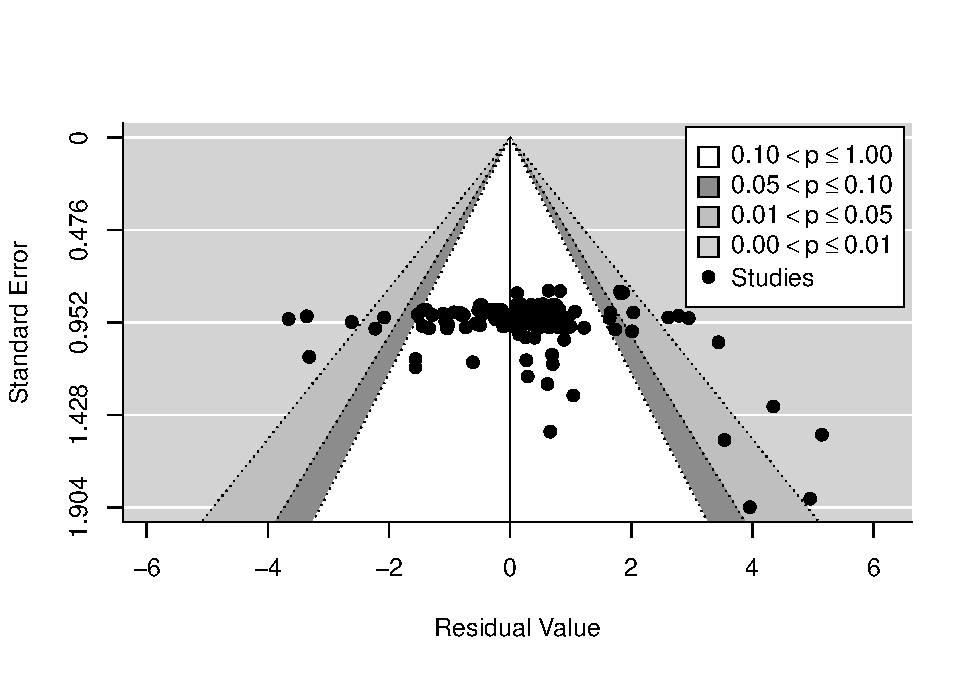
\includegraphics[width=0.9\linewidth]{thesis_files/figure-latex/unnamed-chunk-29-1} 

}

\caption[Funnel plot]{Funnel plot displaying the extracted data points and the distribution of their residuals centered around zero.}\label{fig:unnamed-chunk-29}
\end{figure}
\clearpage
\begin{figure}

{\centering 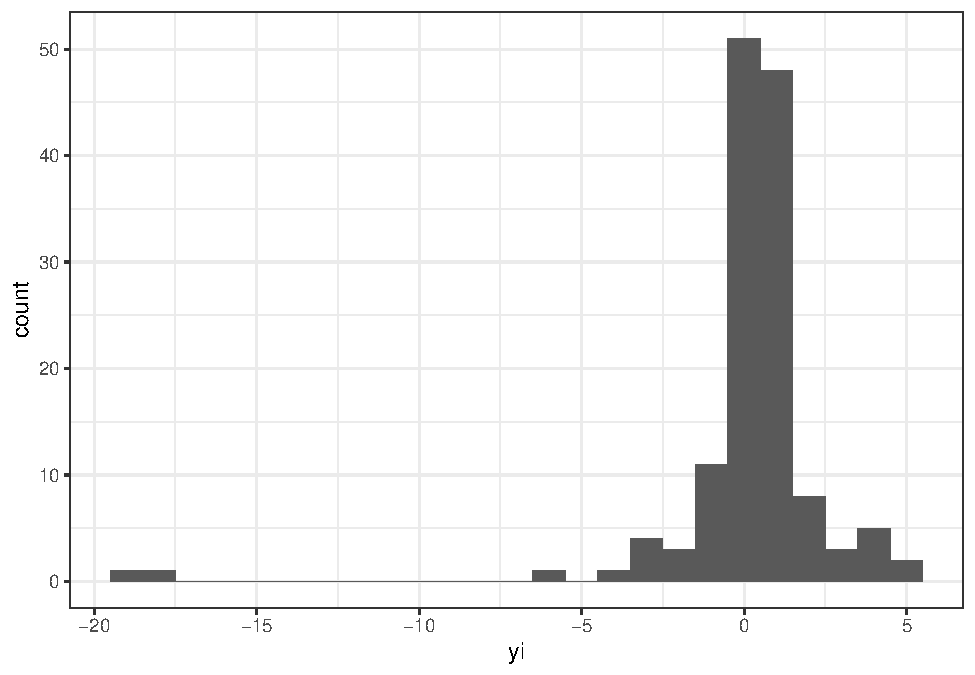
\includegraphics[width=0.9\linewidth]{thesis_files/figure-latex/unnamed-chunk-30-1} 

}

\caption[Histogram of effect sizes]{Distribution of effect sizes (n=140) across data from all 15 studies.}\label{fig:unnamed-chunk-30}
\end{figure}
\begin{table}[!h]

\caption[Thermal stress data by species]{\label{tab:unnamed-chunk-31}TPC metrics extracted from additional papers to collect thermal history data for each species in the meta-analysis (missing data on species X. arvicola, used in Garcia-Ruiz et al 2011)}
\centering
\begin{tabular}[t]{ll>{\raggedright\arraybackslash}p{6cm}}
\toprule
\textbf{Species} & \textbf{Topt (°C)} & \textbf{Reference}\\
\midrule
\cellcolor{gray!6}{Drosophila melanogaster} & \cellcolor{gray!6}{24-26.6°C} & \cellcolor{gray!6}{Klepsatel 2013, David 1988}\\
Leptopilina boulardi & 25°C & De lava et al 2016\\
\cellcolor{gray!6}{Mauremys reevesii} & \cellcolor{gray!6}{37.97 ± 0.64 °C} & \cellcolor{gray!6}{Dang et al 2019}\\
Gryllus firmus & ~30°C & Singh et al 2020\\
\cellcolor{gray!6}{Limnodynastes peronii} & \cellcolor{gray!6}{30°C} & \cellcolor{gray!6}{Seebacher et al 2014}\\
\addlinespace
Limnodynastes tasmaniensis & 30-33°C & Whitehead et al 1989\\
\cellcolor{gray!6}{Platyplectrum ornatum} & \cellcolor{gray!6}{33°C} & \cellcolor{gray!6}{Kern et al 2014}\\
Natrix natrix & ~30°C & Issac 1997\\
\cellcolor{gray!6}{Coturnix japoncia} & \cellcolor{gray!6}{26°C} & \cellcolor{gray!6}{Alagawany et al 2017}\\
Plestiodon chinensis & 33°C & Baojun et al 2010\\
\addlinespace
\cellcolor{gray!6}{Rhodnis prolixus} & \cellcolor{gray!6}{30-35°C} & \cellcolor{gray!6}{Fresquet and Lazzari 2011}\\
Escherichia coli & 37°C, 35-36°C & Doyle and Schoeni 1984, Bronikowski et al 2001\\
\cellcolor{gray!6}{Salmonella} & \cellcolor{gray!6}{35-36°C} & \cellcolor{gray!6}{Bronikowski et al 2001}\\
Caiman latirostris & 32-33°C & Simoncini et al 2019, Parachu-Marco et al 2017, Pina et al 2002\\
\cellcolor{gray!6}{Trachemys scripta} & \cellcolor{gray!6}{32-33°C} & \cellcolor{gray!6}{Dang et al 2019}\\
\addlinespace
Esteya vermicola & 26°C & Wang et al 2015\\
\bottomrule
\end{tabular}
\end{table}
\backmatter

\hypertarget{references}{%
\chapter*{References}\label{references}}
\addcontentsline{toc}{chapter}{References}

\markboth{References}{References}

\noindent

\setlength{\parindent}{-0.20in}
\setlength{\leftskip}{0.20in}
\setlength{\parskip}{8pt}

\hypertarget{refs}{}
\leavevmode\hypertarget{ref-alagawany_heat_2017}{}%
Alagawany, M., Farag, M., Abd El-Hack, M., \& Patra, A. (2017). Heat stress: Effects on productive and reproductive performance of quail. \emph{World's Poultry Science Journal}, \emph{73}(4), 747--756. \url{http://doi.org/10.1017/S0043933917000782}

\leavevmode\hypertarget{ref-amarasekare_intrinsic_2013}{}%
Amarasekare, P., \& Coutinho, R. M. (2013). The intrinsic growth rate as a predictor of population viability under climate warming. \emph{J Anim Ecol}, \emph{82}(6), 1240--1253. \url{http://doi.org/10.1111/1365-2656.12112}

\leavevmode\hypertarget{ref-amarasekare_framework_2012}{}%
Amarasekare, P., \& Savage, V. (2012). A framework for elucidating the temperature dependence of fitness. \emph{The American Naturalist}, \emph{179}(2), 178--191. \url{http://doi.org/10.1086/663677}

\leavevmode\hypertarget{ref-anders_distribution-wide_2006}{}%
Anders, A. D., \& Post, E. (2006). Distribution-wide effects of climate on population densities of a declining migratory landbird. \emph{J Anim Ecology}, \emph{75}(1), 221--227. \url{http://doi.org/10.1111/j.1365-2656.2006.01034.x}

\leavevmode\hypertarget{ref-bambach_seafood_1993}{}%
Bambach, R. K. (1993). Seafood through time: Changes in biomass, energetics, and productivity in the marine ecosystem. \emph{Paleobiology}, \emph{19}(3), 372--397. \url{http://doi.org/10.1017/S0094837300000336}

\leavevmode\hypertarget{ref-baojun_seasonal_2014}{}%
Baojun, S., Wenqi, T., Zhigao, Z., \& Weiguo, D. (2014). The seasonal acclimatisation of locomotion in a terrestrial reptile, plestiodon chinensis(Scincidae). \emph{Asian Herpetological Research}, \emph{5}(3), 197. \url{http://doi.org/10.3724/SP.J.1245.2014.00197}

\leavevmode\hypertarget{ref-bartheld_thermal_2017-2}{}%
Bartheld, J. L., Artacho, P., \& Bacigalupe, L. (2017). Thermal performance curves under daily thermal fluctuation: A study in helmeted water toad tadpoles. \emph{Journal of Thermal Biology}, \emph{70}, 80--85. \url{http://doi.org/10.1016/j.jtherbio.2017.09.008}

\leavevmode\hypertarget{ref-bastille-rousseau_climate_2018}{}%
Bastille-Rousseau, G., Schaefer, J. A., Peers, M. J. L., Ellington, E. H., Mumma, M. A., Rayl, N. D., \ldots{} Murray, D. L. (2018). Climate change can alter predator--prey dynamics and population viability of prey. \emph{Oecologia}, \emph{186}(1), 141--150. \url{http://doi.org/10.1007/s00442-017-4017-y}

\leavevmode\hypertarget{ref-bernardo_biologically_2014}{}%
Bernardo, J. (2014). Biologically grounded predictions of species resistance and resilience to climate change. \emph{Proceedings of the National Academy of Sciences}, \emph{111}(15), 5450--5451. \url{http://doi.org/10.1073/pnas.1404505111}

\leavevmode\hypertarget{ref-bernhardt_life_2020}{}%
Bernhardt, J. R., O'Connor, M. I., Sunday, J. M., \& Gonzalez, A. (2020). Life in fluctuating environments. \emph{Phil. Trans. R. Soc. B}, \emph{375}(1814), 20190454. \url{http://doi.org/10.1098/rstb.2019.0454}

\leavevmode\hypertarget{ref-bernhardt_nonlinear_2018}{}%
Bernhardt, J. R., Sunday, J. M., Thompson, P. L., \& O'Connor, M. I. (2018). Nonlinear averaging of thermal experience predicts population growth rates in a thermally variable environment, 10.

\leavevmode\hypertarget{ref-blankenship_how_2017}{}%
Blankenship, R. E. (2017). How cyanobacteria went green. \emph{Science}, \emph{355}(6332), 1372--1373. \url{http://doi.org/10.1126/science.aam9365}

\leavevmode\hypertarget{ref-bouchard_ecosystem_2014}{}%
Bouchard, F. (2014). Ecosystem evolution is about variation and persistence, not populations and reproduction. \emph{Biol Theory}, \emph{9}(4), 382--391. \url{http://doi.org/10.1007/s13752-014-0171-1}

\leavevmode\hypertarget{ref-bowden_temperature_2018}{}%
Bowden, R. M., \& Paitz, R. T. (2018). Temperature fluctuations and maternal estrogens as critical factors for understanding temperature-dependent sex determination in nature. \emph{J. Exp. Zool.}, \emph{329}(4), 177--184. \url{http://doi.org/10.1002/jez.2183}

\leavevmode\hypertarget{ref-brierley_diel_2014}{}%
Brierley, A. S. (2014). Diel vertical migration. \emph{Current Biology}, \emph{24}(22), R1074--R1076. \url{http://doi.org/10.1016/j.cub.2014.08.054}

\leavevmode\hypertarget{ref-bronikowski_evolutionary_2001}{}%
Bronikowski, A. M., Bennett, A. F., \& Lenski, R. E. (2001). EVOLUTIONARY ADAPTATION TO TEMPERATURE. VIII. EFFECTS OF TEMPERATURE ON GROWTH RATE IN NATURAL ISOLATES OF ESCHERICHIA COLI AND SALMONELLA ENTERICA FROM DIFFERENT THERMAL ENVIRONMENTS. \emph{Evolution}, \emph{55}(1), 33--40. \url{http://doi.org/10.1111/j.0014-3820.2001.tb01270.x}

\leavevmode\hypertarget{ref-brown_toward_2004}{}%
Brown, J. H., Gillooly, J. F., Allen, A. P., Savage, V. M., \& West, G. B. (2004). TOWARD a METABOLIC THEORY OF ECOLOGY. \emph{Ecology}, \emph{85}(7), 1771--1789. \url{http://doi.org/10.1890/03-9000}

\leavevmode\hypertarget{ref-burggren_developmental_2018}{}%
Burggren, W. (2018). Developmental phenotypic plasticity helps bridge stochastic weather events associated with climate change. \emph{Journal of Experimental Biology}, \emph{221}(9), jeb161984. \url{http://doi.org/10.1242/jeb.161984}

\leavevmode\hypertarget{ref-cheung_application_2008}{}%
Cheung, W., Close, C., Lam, V., Watson, R., \& Pauly, D. (2008). Application of macroecological theory to predict effects of climate change on global fisheries potential. \emph{Mar. Ecol. Prog. Ser.}, \emph{365}, 187--197. \url{http://doi.org/10.3354/meps07414}

\leavevmode\hypertarget{ref-clarke_temperature_2006}{}%
Clarke, A. (2006). Temperature and the metabolic theory of ecology. \emph{Funct Ecology}, \emph{20}(2), 405--412. \url{http://doi.org/10.1111/j.1365-2435.2006.01109.x}

\leavevmode\hypertarget{ref-clarke_scaling_1999}{}%
Clarke, A., \& Johnston, N. M. (1999). Scaling of metabolic rate with body mass and temperature in teleost fish. \emph{J Anim Ecology}, \emph{68}(5), 893--905. \url{http://doi.org/10.1046/j.1365-2656.1999.00337.x}

\leavevmode\hypertarget{ref-colinet_mechanisms_2018}{}%
Colinet, H., Rinehart, J. P., Yocum, G. D., \& Greenlee, K. J. (2018). Mechanisms underpinning the beneficial effects of fluctuating thermal regimes in insect cold tolerance. \emph{J Exp Biol}, \emph{221}(14), jeb164806. \url{http://doi.org/10.1242/jeb.164806}

\leavevmode\hypertarget{ref-colinet_insects_2015}{}%
Colinet, H., Sinclair, B. J., Vernon, P., \& Renault, D. (2015). Insects in fluctuating thermal environments. \emph{Annu. Rev. Entomol.}, \emph{60}(1), 123--140. \url{http://doi.org/10.1146/annurev-ento-010814-021017}

\leavevmode\hypertarget{ref-dang_thermal_2019}{}%
Dang, W., Hu, Y.-C., Geng, J., Wang, J., \& Lu, H.-L. (2019). Thermal physiological performance of two freshwater turtles acclimated to different temperatures. \emph{J Comp Physiol B}, \emph{189}(1), 121--130. \url{http://doi.org/10.1007/s00360-018-1194-x}

\leavevmode\hypertarget{ref-delava_effects_2016}{}%
Delava, E., Fleury, F., \& Gibert, P. (2016). Effects of daily fluctuating temperatures on the drosophila--leptopilina boulardi parasitoid association. \emph{Journal of Thermal Biology}, \emph{60}, 95--102. \url{http://doi.org/10.1016/j.jtherbio.2016.06.012}

\leavevmode\hypertarget{ref-delmas_mechanistic_2007}{}%
Delmas, V., Prevot-Julliard, A.-C., Pieau, C., \& Girondot, M. (2007). A mechanistic model of temperature-dependent sex determination in a chelonian: The european pond turtle. \emph{Funct Ecology}, \emph{0}(0), 071027215958001--??? \url{http://doi.org/10.1111/j.1365-2435.2007.01349.x}

\leavevmode\hypertarget{ref-dempster_fluctuations_1981}{}%
Dempster, J. P., \& Pollard, E. (1981). Fluctuations in resource availability and insect populations. \emph{Oecologia}, \emph{50}(3), 412--416. \url{http://doi.org/10.1007/BF00344984}

\leavevmode\hypertarget{ref-descamps-julien_stable_2005}{}%
Descamps-Julien, B., \& Gonzalez, A. (2005). STABLE COEXISTENCE IN a FLUCTUATING ENVIRONMENT: AN EXPERIMENTAL DEMONSTRATION. \emph{Ecology}, \emph{86}(10), 2815--2824. \url{http://doi.org/10.1890/04-1700}

\leavevmode\hypertarget{ref-dobramysl_environmental_2013}{}%
Dobramysl, U., \& Tauber, U. C. (2013). Environmental vs. Demographic variability in two-species predator-prey models. \emph{Phys. Rev. Lett.}, \emph{110}(4), 048105. \url{http://doi.org/10.1103/PhysRevLett.110.048105}

\leavevmode\hypertarget{ref-dowd_thermal_2015}{}%
Dowd, W. W., King, F. A., \& Denny, M. W. (2015). Thermal variation, thermal extremes and the physiological performance of individuals. \emph{Journal of Experimental Biology}, \emph{218}(12), 1956--1967. \url{http://doi.org/10.1242/jeb.114926}

\leavevmode\hypertarget{ref-doyle_survival_1984}{}%
Doyle, M. P., \& Schoeni, J. L. (1984). Survival and growth characteristics of escherichia coli associated with hemorrhagic colitis. \emph{Applied and Environmental Microbiology}, \emph{48}(4), 855--856. \url{http://doi.org/10.1128/AEM.48.4.855-856.1984}

\leavevmode\hypertarget{ref-du_embryonic_2009}{}%
Du, W.-G., Shen, J.-W., \& Wang, L. (2009). Embryonic development rate and hatchling phenotypes in the chinese three-keeled pond turtle (chinemys reevesii): The influence of fluctuating temperature versus constant temperature. \emph{Journal of Thermal Biology}, \emph{34}(5), 250--255. \url{http://doi.org/10.1016/j.jtherbio.2009.03.002}

\leavevmode\hypertarget{ref-farhang-sardroodi_environmental_2019}{}%
Farhang-Sardroodi, S., Darooneh, A. H., Kohandel, M., \& Komarova, N. L. (2019). Environmental spatial and temporal variability and its role in non-favoured mutant dynamics. \emph{J. R. Soc. Interface.}, \emph{16}(157), 20180781. \url{http://doi.org/10.1098/rsif.2018.0781}

\leavevmode\hypertarget{ref-fresquet_response_2011}{}%
Fresquet, N., \& Lazzari, C. R. (2011). Response to heat in rhodnius prolixus: The role of the thermal background. \emph{Journal of Insect Physiology}, \emph{57}(10), 1446--1449. \url{http://doi.org/10.1016/j.jinsphys.2011.07.012}

\leavevmode\hypertarget{ref-garcia-ruiz_effects_2011}{}%
García-Ruiz, E., Marco, V., \& Pérez-Moreno, I. (2011). Effects of variable and constant temperatures on the embryonic development and survival of a new grape pest, xylotrechus arvicola (coleoptera: Cerambycidae). \emph{Environ Entomol}, \emph{40}(4), 939--947. \url{http://doi.org/10.1603/EN11080}

\leavevmode\hypertarget{ref-gillooly_response_2006}{}%
Gillooly, J. F., Allen, A. P., Savage, V. M., Charnov, E. L., West, G. B., \& Brown, J. H. (2006). Response to clarke and fraser: Effects of temperature on metabolic rate. \emph{Funct Ecology}, \emph{20}(2), 400--404. \url{http://doi.org/10.1111/j.1365-2435.2006.01110.x}

\leavevmode\hypertarget{ref-glass_should_2019}{}%
Glass, J. R., \& Stahlschmidt, Z. R. (2019). Should i stay or should i go? Complex environments influence the developmental plasticity of flight capacity and flight-related trade-offs. \emph{Biological Journal of the Linnean Society}, \emph{128}(1), 59--69. \url{http://doi.org/10.1093/biolinnean/blz073}

\leavevmode\hypertarget{ref-gudmundson_environmental_2015}{}%
Gudmundson, S., Eklöf, A., \& Wennergren, U. (2015). Environmental variability uncovers disruptive effects of species' interactions on population dynamics. \emph{Proc. R. Soc. B.}, \emph{282}(1812), 20151126. \url{http://doi.org/10.1098/rspb.2015.1126}

\leavevmode\hypertarget{ref-guralnick_evolutionary_2007}{}%
Guralnick, L. J., Cline, A., Smith, M., \& Sage, R. F. (2007). Evolutionary physiology: The extent of c4 and CAM photosynthesis in the genera anacampseros and grahamia of the portulacaceae. \emph{Journal of Experimental Botany}, \emph{59}(7), 1735--1742. \url{http://doi.org/10.1093/jxb/ern081}

\leavevmode\hypertarget{ref-helmuth_organismal_2010}{}%
Helmuth, B., Broitman, B. R., Yamane, L., Gilman, S. E., Mach, K., Mislan, K. A. S., \& Denny, M. W. (2010). Organismal climatology: Analyzing environmental variability at scales relevant to physiological stress. \emph{Journal of Experimental Biology}, \emph{213}(6), 995--1003. \url{http://doi.org/10.1242/jeb.038463}

\leavevmode\hypertarget{ref-higgins_cochrane_2011}{}%
Higgins, J., Thomas, J., Chandler, J., Li, T., Page, M., \& Welch, V. (2011). \emph{Cochrane handbook for systematic reviews of interventions} (Vol. 5.1.0). Retrieved from \url{www.training.cochrane.org/handbook}

\leavevmode\hypertarget{ref-holmes_robust_2016}{}%
Holmes, C. R., Woollings, T., Hawkins, E., \& Vries, H. de. (2016). Robust future changes in temperature variability under greenhouse gas forcing and the relationship with thermal advection. \emph{Journal of Climate}, \emph{29}(6), 2221--2236. \url{http://doi.org/10.1175/JCLI-D-14-00735.1}

\leavevmode\hypertarget{ref-holt_impacts_2003}{}%
Holt, R. D., Barfield, M., \& Gonzalez, A. (2003). Impacts of environmental variability in open populations and communities: ``Inflation'' in sink environments. \emph{Theoretical Population Biology}, \emph{64}(3), 315--330. \url{http://doi.org/10.1016/S0040-5809(03)00087-X}

\leavevmode\hypertarget{ref-horne_spatial_1995}{}%
Horne, J. K., \& Schneider, D. C. (1995). Spatial variance in ecology. \emph{Oikos}, \emph{74}(1), 18. \url{http://doi.org/10.2307/3545670}

\leavevmode\hypertarget{ref-huey_behavioral_1974}{}%
Huey, R. B. (1974). Behavioral thermoregulation in lizards: Importance of associated costs. \emph{Science}, \emph{184}(4140), 1001--1003. \url{http://doi.org/10.1126/science.184.4140.1001}

\leavevmode\hypertarget{ref-huey_physiological_1990}{}%
Huey, R. B., \& Bennett, A. F. (1990). Physiological adjustments to fluctuating thermal environments: An ecological and evolutionary perspective. \emph{Stress Proteins in Biology and Medicine}, 23.

\leavevmode\hypertarget{ref-huey_predicting_2012}{}%
Huey, R. B., Kearney, M. R., Krockenberger, A., Holtum, J. A. M., Jess, M., \& Williams, S. E. (2012). Predicting organismal vulnerability to climate warming: Roles of behaviour, physiology and adaptation. \emph{Phil. Trans. R. Soc. B}, \emph{367}(1596), 1665--1679. \url{http://doi.org/10.1098/rstb.2012.0005}

\leavevmode\hypertarget{ref-husak_how_2017}{}%
Husak, J. F., \& Lailvaux, S. P. (2017). How do we measure the cost of whole-organism performance traits? \emph{Integrative and Comparative Biology}, \emph{57}(2), 333--343. \url{http://doi.org/10.1093/icb/icx048}

\leavevmode\hypertarget{ref-isaac_isaac_2003pdf_2003}{}%
Isaac, L. A. (2003). Isaac\_2003.pdf. University of Victoria. Retrieved from \url{https://dspace.library.uvic.ca/handle/1828/356}

\leavevmode\hypertarget{ref-kearney_potential_2009}{}%
Kearney, M., Shine, R., \& Porter, W. P. (2009). The potential for behavioral thermoregulation to buffer "cold-blooded" animals against climate warming. \emph{Proceedings of the National Academy of Sciences}, \emph{106}(10), 3835--3840. \url{http://doi.org/10.1073/pnas.0808913106}

\leavevmode\hypertarget{ref-kern_temperature_2014}{}%
Kern, P., Cramp, R. L., \& Franklin, C. E. (2014). Temperature and UV-b-insensitive performance in tadpoles of the ornate burrowing frog: An ephemeral pond specialist. \emph{Journal of Experimental Biology}, \emph{217}(8), 1246--1252. \url{http://doi.org/10.1242/jeb.097006}

\leavevmode\hypertarget{ref-kern_physiological_2015-3}{}%
Kern, P., Cramp, R. L., \& Franklin, C. E. (2015). Physiological responses of ectotherms to daily temperature variation. \emph{Journal of Experimental Biology}, \emph{218}(19), 3068--3076. \url{http://doi.org/10.1242/jeb.123166}

\leavevmode\hypertarget{ref-khelifa_usefulness_2019}{}%
Khelifa, R., Blanckenhorn, W. U., Roy, J., Rohner, P. T., \& Mahdjoub, H. (2019). Usefulness and limitations of thermal performance curves in predicting ectotherm development under climatic variability. \emph{J Anim Ecol}, \emph{88}(12), 1901--1912. \url{http://doi.org/10.1111/1365-2656.13077}

\leavevmode\hypertarget{ref-klepsatel_variation_2013}{}%
Klepsatel, P., Gáliková, M., De Maio, N., Huber, C. D., Schlötterer, C., \& Flatt, T. (2013). VARIATION IN THERMAL PERFORMANCE AND REACTION NORMS AMONG POPULATIONS OF \emph{DROSOPHILA MELANOGASTER}: THERMAL PERFORMANCE IN DROSOPHILA. \emph{Evolution}, \emph{67}(12), 3573--3587. \url{http://doi.org/10.1111/evo.12221}

\leavevmode\hypertarget{ref-knoll_chapter_2008}{}%
Knoll, A. (2008). Chapter 1. In \emph{Cyanobacteria and earth history}.

\leavevmode\hypertarget{ref-kremer_gradual_2018}{}%
Kremer, C. T., Fey, S. B., Arellano, A. A., \& Vasseur, D. A. (2018). Gradual plasticity alters population dynamics in variable environments: Thermal acclimation in the green alga \emph{chlamydomonas reinhartdii}. \emph{Proc. R. Soc. B.}, \emph{285}(1870), 20171942. \url{http://doi.org/10.1098/rspb.2017.1942}

\leavevmode\hypertarget{ref-krenek_coping_2012}{}%
Krenek, S., Petzoldt, T., \& Berendonk, T. U. (2012). Coping with temperature at the warm edge -- patterns of thermal adaptation in the microbial eukaryote paramecium caudatum. \emph{PLoS ONE}, \emph{7}(3), e30598. \url{http://doi.org/10.1371/journal.pone.0030598}

\leavevmode\hypertarget{ref-kroeker_ecological_2020}{}%
Kroeker, K. J., Bell, L. E., Donham, E. M., Hoshijima, U., Lummis, S., Toy, J. A., \& Willis‐Norton, E. (2020). Ecological change in dynamic environments: Accounting for temporal environmental variability in studies of ocean change biology. \emph{Glob Change Biol}, \emph{26}(1), 54--67. \url{http://doi.org/10.1111/gcb.14868}

\leavevmode\hypertarget{ref-lampert_adaptive_1989}{}%
Lampert, W. (1989). The adaptive significance of diel vertical migration of zooplankton. \emph{Functional Ecology}, \emph{3}(1), 21. \url{http://doi.org/10.2307/2389671}

\leavevmode\hypertarget{ref-lawson_environmental_2015}{}%
Lawson, C. R., Vindenes, Y., Bailey, L., \& Pol, M. van de. (2015). Environmental variation and population responses to global change. \emph{Ecol Lett}, \emph{18}(7), 724--736. \url{http://doi.org/10.1111/ele.12437}

\leavevmode\hypertarget{ref-lowenborg_how_2012}{}%
Löwenborg, K., Gotthard, K., \& Hagman, M. (2012). How a thermal dichotomy in nesting environments influences offspring of the world's most northerly oviparous snake, \emph{natrix natrix} (colubridae): Grass snake nest-site dichotomy. \emph{Biol J Linn Soc Lond}, \emph{107}(4), 833--844. \url{http://doi.org/10.1111/j.1095-8312.2012.01972.x}

\leavevmode\hypertarget{ref-manenti_predictability_2014-2}{}%
Manenti, T., Sørensen, J. G., Moghadam, N. N., \& Loeschcke, V. (2014). Predictability rather than amplitude of temperature fluctuations determines stress resistance in a natural population of \emph{drosophila simulans}. \emph{J. Evol. Biol.}, \emph{27}(10), 2113--2122. \url{http://doi.org/10.1111/jeb.12463}

\leavevmode\hypertarget{ref-massey_measurement_2019}{}%
Massey, M. D., Holt, S. M., Brooks, R. J., \& Rollinson, N. (2019). Measurement and modelling of primary sex ratios for species with temperature-dependent sex determination. \emph{J Exp Biol}, \emph{222}(1), jeb190215. \url{http://doi.org/10.1242/jeb.190215}

\leavevmode\hypertarget{ref-morison_light_2020}{}%
Morison, F., Franzè, G., Harvey, E., \& Menden‐Deuer, S. (2020). Light fluctuations are key in modulating plankton trophic dynamics and their impact on primary production. \emph{Limnol Oceanogr}, \emph{5}(5), 346--353. \url{http://doi.org/10.1002/lol2.10156}

\leavevmode\hypertarget{ref-moyano_effects_2017}{}%
Moyano, M., Candebat, C., Ruhbaum, Y., Álvarez-Fernández, S., Claireaux, G., Zambonino-Infante, J.-L., \& Peck, M. A. (2017). Effects of warming rate, acclimation temperature and ontogeny on the critical thermal maximum of temperate marine fish larvae. \emph{PLoS ONE}, \emph{12}(7), e0179928. \url{http://doi.org/10.1371/journal.pone.0179928}

\leavevmode\hypertarget{ref-noble_developmental_2018}{}%
Noble, D. W. A., Stenhouse, V., \& Schwanz, L. E. (2018). Developmental temperatures and phenotypic plasticity in reptiles: A systematic review and meta-analysis: Incubation temperature and plasticity. \emph{Biol Rev}, \emph{93}(1), 72--97. \url{http://doi.org/10.1111/brv.12333}

\leavevmode\hypertarget{ref-paaijmans_temperature_2013}{}%
Paaijmans, K. P., Heinig, R. L., Seliga, R. A., Blanford, J. I., Blanford, S., Murdock, C. C., \& Thomas, M. B. (2013). Temperature variation makes ectotherms more sensitive to climate change. \emph{Glob Change Biol}, \emph{19}(8), 2373--2380. \url{http://doi.org/10.1111/gcb.12240}

\leavevmode\hypertarget{ref-parachu_marco_new_2017}{}%
Parachu Marco, M. V., Leiva, P., Iungman, J. L., Simonici, M. S., \& Pina, C. I. (2017). New evidence characterizing temperature-dependent sex determination in broad-snouted caiman, caiman latirostris. \emph{Herpetological Conservation and Biology}, (12), 78--84.

\leavevmode\hypertarget{ref-parepa_environmental_2013}{}%
Parepa, M., Fischer, M., \& Bossdorf, O. (2013). Environmental variability promotes plant invasion. \emph{Nat Commun}, \emph{4}(1), 1604. \url{http://doi.org/10.1038/ncomms2632}

\leavevmode\hypertarget{ref-pendlebury_variation_2004-1}{}%
Pendlebury, C. J. (2004). Variation in temperature increases the cost of living in birds. \emph{Journal of Experimental Biology}, \emph{207}(12), 2065--2070. \url{http://doi.org/10.1242/jeb.00999}

\leavevmode\hypertarget{ref-petchey_environmental_2000}{}%
Petchey, O. L. (2000). Environmental colour affects aspects of single--species population dynamics. \emph{Proc. R. Soc. Lond. B}, \emph{267}(1445), 747--754. \url{http://doi.org/10.1098/rspb.2000.1066}

\leavevmode\hypertarget{ref-pina_effect_2003}{}%
Piña, C. I., Larriera, A., \& Cabrera, M. R. (2003). Effect of incubation temperature on incubation period, sex ratio, hatching success, and survivorship in caiman latirostris (crocodylia, alligatoridae). \emph{Journal of Herpetology}, \emph{37}(1), 199--202. \href{http://doi.org/10.1670/0022-1511(2003)037\%5B0199:EOITOI\%5D2.0.CO;2}{http://doi.org/10.1670/0022-1511(2003)037{[}0199:EOITOI{]}2.0.CO;2}

\leavevmode\hypertarget{ref-portner_ecology_2008}{}%
Portner, H. O., \& Farrell, A. P. (2008). ECOLOGY: Physiology and climate change. \emph{Science}, \emph{322}(5902), 690--692. \url{http://doi.org/10.1126/science.1163156}

\leavevmode\hypertarget{ref-qu_incubation_2014}{}%
Qu, Y.-F., Lu, H.-L., Li, H., \& Ji, X. (2014). Incubation temperature fluctuation does not affect incubation length and hatchling phenotype in the chinese skink plestiodon chinensis. \emph{Journal of Thermal Biology}, \emph{46}, 10--15. \url{http://doi.org/10.1016/j.jtherbio.2014.09.008}

\leavevmode\hypertarget{ref-reed_phenotypic_2010}{}%
Reed, T. E., Waples, R. S., Schindler, D. E., Hard, J. J., \& Kinnison, M. T. (2010). Phenotypic plasticity and population viability: The importance of environmental predictability. \emph{Proc. R. Soc. B.}, \emph{277}(1699), 3391--3400. \url{http://doi.org/10.1098/rspb.2010.0771}

\leavevmode\hypertarget{ref-rolandi_costs_2018}{}%
Rolandi, C., \& Schilman, P. E. (2018). The costs of living in a thermal fluctuating environment for the tropical haematophagous bug, rhodnius prolixus. \emph{Journal of Thermal Biology}, \emph{74}, 92--99. \url{http://doi.org/10.1016/j.jtherbio.2018.03.022}

\leavevmode\hypertarget{ref-romanuk_environmental_2002}{}%
Romanuk, T. N., \& Kolasa, J. (2002). Environmental variability alters the relationship between richness and variability of community abundances in aquatic rock pool microcosms. \emph{Écoscience}, \emph{9}(1), 55--62. \url{http://doi.org/10.1080/11956860.2002.11682690}

\leavevmode\hypertarget{ref-ruel_jensens_1999}{}%
Ruel, J. J., \& Ayres, M. P. (1999). Jensen's inequality predicts effects of environmental variation. \emph{Trends in Ecology \& Evolution}, \emph{14}(9), 361--366. \url{http://doi.org/10.1016/S0169-5347(99)01664-X}

\leavevmode\hypertarget{ref-russill_tipping_2009}{}%
Russill, C., \& Nyssa, Z. (2009). The tipping point trend in climate change communication. \emph{Global Environmental Change}, \emph{19}(3), 336--344. \url{http://doi.org/10.1016/j.gloenvcha.2009.04.001}

\leavevmode\hypertarget{ref-saxon_temperature_2018-1}{}%
Saxon, A. D., O'Brien, E. K., \& Bridle, J. R. (2018). Temperature fluctuations during development reduce male fitness and may limit adaptive potential in tropical rainforest \emph{drosophila}. \emph{J. Evol. Biol.}, \emph{31}(3), 405--415. \url{http://doi.org/10.1111/jeb.13231}

\leavevmode\hypertarget{ref-seebacher_embryonic_2014}{}%
Seebacher, F., \& Grigaltchik, V. S. (2014). Embryonic developmental temperatures modulate thermal acclimation of performance curves in tadpoles of the frog limnodynastes peronii. \emph{PLoS ONE}, \emph{9}(9), e106492. \url{http://doi.org/10.1371/journal.pone.0106492}

\leavevmode\hypertarget{ref-semenov_influence_2007}{}%
Semenov, A. V., Van Bruggen, A. H., Van Overbeek, L., Termorshuizen, A. J., \& Semenov, A. M. (2007). Influence of temperature fluctuations on escherichia coli o157:H7 and salmonella enterica serovar typhimurium in cow manure: Effect of temperature fluctuation on human pathogens. \emph{FEMS Microbiology Ecology}, \emph{60}(3), 419--428. \url{http://doi.org/10.1111/j.1574-6941.2007.00306.x}

\leavevmode\hypertarget{ref-simoncini_influence_2019}{}%
Simoncini, M. S., Leiva, P. M., Piña, C. I., \& Cruz, F. B. (2019). Influence of temperature variation on incubation period, hatching success, sex ratio, and phenotypes in \emph{caiman latirostris}: SIMONCINI \textless{}span style="font-variant:Small-caps;"\textgreater{}et al.\textless{}/span\textgreater{}. \emph{J. Exp. Zool.}, \emph{331}(5), 299--307. \url{http://doi.org/10.1002/jez.2265}

\leavevmode\hypertarget{ref-singh_effect_2020}{}%
Singh, R., Prathibha, P., \& Jain, M. (2020). \emph{Effect of temperature on life-history traits and mating calls of a field cricket, \textup{acanthogryllus asiaticus}} (preprint). Ecology. Retrieved from \url{http://biorxiv.org/lookup/doi/10.1101/2020.06.06.137869}

\leavevmode\hypertarget{ref-sommer_paradox_1984}{}%
Sommer, U. (1984). The paradox of the plankton: Fluctuations of phosphorus availability maintain diversity of phytoplankton in flow-through cultures1. \emph{Limnol. Oceanogr.}, \emph{29}(3), 633--636. \url{http://doi.org/10.4319/lo.1984.29.3.0633}

\leavevmode\hypertarget{ref-soo_origins_2017}{}%
Soo, R. M., Hemp, J., Parks, D. H., Fischer, W. W., \& Hugenholtz, P. (2017). On the origins of oxygenic photosynthesis and aerobic respiration in cyanobacteria. \emph{Science}, \emph{355}(6332), 1436--1440. \url{http://doi.org/10.1126/science.aal3794}

\leavevmode\hypertarget{ref-stewart_mesocosm_2013}{}%
Stewart, R. I., Dossena, M., Bohan, D. A., Jeppesen, E., Kordas, R. L., Ledger, M. E., \ldots{} Woodward, G. (2013). Mesocosm experiments as a tool for ecological climate-change research. In \emph{Advances in ecological research} (Vol. 48, pp. 71--181). Elsevier. \url{http://doi.org/10.1016/B978-0-12-417199-2.00002-1}

\leavevmode\hypertarget{ref-sunday_thermal_2012}{}%
Sunday, J. M., Bates, A. E., \& Dulvy, N. K. (2012). Thermal tolerance and the global redistribution of animals. \emph{Nature Clim Change}, \emph{2}(9), 686--690. \url{http://doi.org/10.1038/nclimate1539}

\leavevmode\hypertarget{ref-tabari_shift_2012}{}%
Tabari, H., Hosseinzadeh Talaee, P., Ezani, A., \& Shifteh Some'e, B. (2012). Shift changes and monotonic trends in autocorrelated temperature series over iran. \emph{Theor Appl Climatol}, \emph{109}(1), 95--108. \url{http://doi.org/10.1007/s00704-011-0568-8}

\leavevmode\hypertarget{ref-treidel_temperature_2016-1}{}%
Treidel, L. A., Carter, A. W., \& Bowden, R. M. (2016). Temperature experienced during incubation affects antioxidant capacity but not oxidative damage in hatchling red-eared slider turtles ( \emph{trachemys scripta elegans} ). \emph{J Exp Biol}, \emph{219}(4), 561--570. \url{http://doi.org/10.1242/jeb.128843}

\leavevmode\hypertarget{ref-tuff_framework_2016}{}%
Tuff, K. T., Tuff, T., \& Davies, K. F. (2016). A framework for integrating thermal biology into fragmentation research. \emph{Ecol Lett}, \emph{19}(4), 361--374. \url{http://doi.org/10.1111/ele.12579}

\leavevmode\hypertarget{ref-vasseur_increased_2014}{}%
Vasseur, D. A., DeLong, J. P., Gilbert, B., Greig, H. S., Harley, C. D. G., McCann, K. S., \ldots{} O'Connor, M. I. (2014). Increased temperature variation poses a greater risk to species than climate warming. \emph{Proc. R. Soc. B.}, \emph{281}(1779), 20132612. \url{http://doi.org/10.1098/rspb.2013.2612}

\leavevmode\hypertarget{ref-vasseur_phase-locking_2009}{}%
Vasseur, D. A., \& Fox, J. W. (2009). Phase-locking and environmental fluctuations generate synchrony in a predator--prey community. \emph{Nature}, \emph{460}(7258), 1007--1010. \url{http://doi.org/10.1038/nature08208}

\leavevmode\hypertarget{ref-vasseur_color_2004}{}%
Vasseur, D. A., \& Yodzis, P. (2004). THE COLOR OF ENVIRONMENTAL NOISE. \emph{Ecology}, \emph{85}(4), 1146--1152. \url{http://doi.org/10.1890/02-3122}

\leavevmode\hypertarget{ref-viechtbauer_conducting_2010}{}%
Viechtbauer, W. (2010). Conducting meta-analyses in \emph{r} with the \textbf{metafor} package. \emph{J. Stat. Soft.}, \emph{36}(3). \url{http://doi.org/10.18637/jss.v036.i03}

\leavevmode\hypertarget{ref-wang_effects_2015}{}%
Wang, Y.-b., Pang, W.-x., Yv, X.-n., Li, J.-j., Zhang, Y.-a., \& Sung, C.-k. (2015). The effects of fluctuating culture temperature on stress tolerance and antioxidase expression in esteya vermicola. \emph{J Microbiol.}, \emph{53}(2), 122--126. \url{http://doi.org/10.1007/s12275-015-4529-2}

\leavevmode\hypertarget{ref-west_allometric_2002}{}%
West, G. B., Woodruff, W. H., \& Brown, J. H. (2002). Allometric scaling of metabolic rate from molecules and mitochondria to cells and mammals. \emph{Proceedings of the National Academy of Sciences}, \emph{99}(Supplement 1), 2473--2478. \url{http://doi.org/10.1073/pnas.012579799}

\leavevmode\hypertarget{ref-whitehead_effect_1989}{}%
Whitehead, P. J., Puckridge, J. T., Leigh, C. M., \& Seymour, R. S. (1989). Effect of temperature on jump performance of the frog \emph{limnodynastes tasmaniensis}. \emph{Physiological Zoology}, \emph{62}(4), 937--949. \url{http://doi.org/10.1086/physzool.62.4.30157938}

\leavevmode\hypertarget{ref-wigley_anthropogenic_1998-1}{}%
Wigley, T. M. (1998). Anthropogenic influence on the autocorrelation structure of hemispheric-mean temperatures. \emph{Science}, \emph{282}(5394), 1676--1679. \url{http://doi.org/10.1126/science.282.5394.1676}

\leavevmode\hypertarget{ref-yoshida_rapid_2003}{}%
Yoshida, T., Jones, L. E., Ellner, S. P., Fussmann, G. F., \& Hairston, N. G. (2003). Rapid evolution drives ecological dynamics in a predator--prey system. \emph{Nature}, \emph{424}(6946), 303--306. \url{http://doi.org/10.1038/nature01767}


% Index?

\end{document}
